\documentclass[twoside]{book}

% Packages required by doxygen
\usepackage{fixltx2e}
\usepackage{calc}
\usepackage{doxygen}
\usepackage[export]{adjustbox} % also loads graphicx
\usepackage{graphicx}
\usepackage[utf8]{inputenc}
\usepackage{makeidx}
\usepackage{multicol}
\usepackage{multirow}
\PassOptionsToPackage{warn}{textcomp}
\usepackage{textcomp}
\usepackage[nointegrals]{wasysym}
\usepackage[table]{xcolor}

% NLS support packages
\usepackage[spanish]{babel}
% Font selection
\usepackage[T1]{fontenc}
\usepackage[scaled=.90]{helvet}
\usepackage{courier}
\usepackage{amssymb}
\usepackage{sectsty}
\renewcommand{\familydefault}{\sfdefault}
\allsectionsfont{%
  \fontseries{bc}\selectfont%
  \color{darkgray}%
}
\renewcommand{\DoxyLabelFont}{%
  \fontseries{bc}\selectfont%
  \color{darkgray}%
}
\newcommand{\+}{\discretionary{\mbox{\scriptsize$\hookleftarrow$}}{}{}}

% Page & text layout
\usepackage{geometry}
\geometry{%
  a4paper,%
  top=2.5cm,%
  bottom=2.5cm,%
  left=2.5cm,%
  right=2.5cm%
}
\tolerance=750
\hfuzz=15pt
\hbadness=750
\setlength{\emergencystretch}{15pt}
\setlength{\parindent}{0cm}
\setlength{\parskip}{3ex plus 2ex minus 2ex}
\makeatletter
\renewcommand{\paragraph}{%
  \@startsection{paragraph}{4}{0ex}{-1.0ex}{1.0ex}{%
    \normalfont\normalsize\bfseries\SS@parafont%
  }%
}
\renewcommand{\subparagraph}{%
  \@startsection{subparagraph}{5}{0ex}{-1.0ex}{1.0ex}{%
    \normalfont\normalsize\bfseries\SS@subparafont%
  }%
}
\makeatother

% Headers & footers
\usepackage{fancyhdr}
\pagestyle{fancyplain}
\fancyhead[LE]{\fancyplain{}{\bfseries\thepage}}
\fancyhead[CE]{\fancyplain{}{}}
\fancyhead[RE]{\fancyplain{}{\bfseries\leftmark}}
\fancyhead[LO]{\fancyplain{}{\bfseries\rightmark}}
\fancyhead[CO]{\fancyplain{}{}}
\fancyhead[RO]{\fancyplain{}{\bfseries\thepage}}
\fancyfoot[LE]{\fancyplain{}{}}
\fancyfoot[CE]{\fancyplain{}{}}
\fancyfoot[RE]{\fancyplain{}{\bfseries\scriptsize Generado por Doxygen }}
\fancyfoot[LO]{\fancyplain{}{\bfseries\scriptsize Generado por Doxygen }}
\fancyfoot[CO]{\fancyplain{}{}}
\fancyfoot[RO]{\fancyplain{}{}}
\renewcommand{\footrulewidth}{0.4pt}
\renewcommand{\chaptermark}[1]{%
  \markboth{#1}{}%
}
\renewcommand{\sectionmark}[1]{%
  \markright{\thesection\ #1}%
}

% Indices & bibliography
\usepackage{natbib}
\usepackage[titles]{tocloft}
\setcounter{tocdepth}{3}
\setcounter{secnumdepth}{5}
\makeindex

% Hyperlinks (required, but should be loaded last)
\usepackage{ifpdf}
\ifpdf
  \usepackage[pdftex,pagebackref=true]{hyperref}
\else
  \usepackage[ps2pdf,pagebackref=true]{hyperref}
\fi
\hypersetup{%
  colorlinks=true,%
  linkcolor=blue,%
  citecolor=blue,%
  unicode%
}

% Custom commands
\newcommand{\clearemptydoublepage}{%
  \newpage{\pagestyle{empty}\cleardoublepage}%
}

\usepackage{caption}
\captionsetup{labelsep=space,justification=centering,font={bf},singlelinecheck=off,skip=4pt,position=top}

%===== C O N T E N T S =====

\begin{document}

% Titlepage & ToC
\hypersetup{pageanchor=false,
             bookmarksnumbered=true,
             pdfencoding=unicode
            }
\pagenumbering{alph}
\begin{titlepage}
\vspace*{7cm}
\begin{center}%
{\Large Gestión de una terminal de contenedores de carga. \\[1ex]\large version 1 01/11/2020 }\\
\vspace*{1cm}
{\large Generado por Doxygen 1.8.13}\\
\end{center}
\end{titlepage}
\clearemptydoublepage
\pagenumbering{roman}
\tableofcontents
\clearemptydoublepage
\pagenumbering{arabic}
\hypersetup{pageanchor=true}

%--- Begin generated contents ---
\chapter{Gestión de una terminal de contenedores de carga.}
\label{index}\hypertarget{index}{}En este ejemplo se construye un programa modular que ofrece un menú de opciones para gestionar una lavadora. Se introducen las clases {\itshape \hyperlink{class_lavadora}{Lavadora}}, {\itshape \hyperlink{class_cubeta}{Cubeta}} y {\itshape \hyperlink{class_prenda}{Prenda}}.

Sólo se documentan elementos públicos. En una próxima sesión se verá un ejemplo de proyecto completamente documentado, incluyendo los elementos privados. 
\chapter{Índice de clases}
\section{Lista de clases}
Lista de las clases, estructuras, uniones e interfaces con una breve descripción\+:\begin{DoxyCompactList}
\item\contentsline{section}{\hyperlink{class_almacenaje}{Almacenaje} \\*Representa un area de almacenaje de una terminal de contenedores de carga }{\pageref{class_almacenaje}}{}
\item\contentsline{section}{\hyperlink{class_contenedor}{Contenedor} \\*Representa un contenidor amb una matrícula i una longitud }{\pageref{class_contenedor}}{}
\item\contentsline{section}{\hyperlink{class_espera}{Espera} \\*Representa un area de espera de una terminal de contenedores de carga }{\pageref{class_espera}}{}
\item\contentsline{section}{\hyperlink{class_segmento}{Segmento} \\*Representa un segment amb una ubicació i una longitud }{\pageref{class_segmento}}{}
\item\contentsline{section}{\hyperlink{class_terminal}{Terminal} \\*Representa una \hyperlink{class_terminal}{Terminal} de contenedores de carga }{\pageref{class_terminal}}{}
\item\contentsline{section}{\hyperlink{class_ubicacion}{Ubicacion} \\*Representa una ubicació en una terminal amb 3 coordenades }{\pageref{class_ubicacion}}{}
\end{DoxyCompactList}

\chapter{Indice de archivos}
\section{Lista de archivos}
Lista de todos los archivos con descripciones breves\+:\begin{DoxyCompactList}
\item\contentsline{section}{\hyperlink{_cubeta_8hh}{Cubeta.\+hh} \\*Especificación de la clase \hyperlink{class_cubeta}{Cubeta} }{\pageref{_cubeta_8hh}}{}
\item\contentsline{section}{\hyperlink{_lavadora_8hh}{Lavadora.\+hh} \\*Especificación de la clase \hyperlink{class_lavadora}{Lavadora} }{\pageref{_lavadora_8hh}}{}
\item\contentsline{section}{\hyperlink{_prenda_8hh}{Prenda.\+hh} \\*Especificación de la clase \hyperlink{class_prenda}{Prenda} }{\pageref{_prenda_8hh}}{}
\item\contentsline{section}{\hyperlink{pro2__especif_8cc}{pro2\+\_\+especif.\+cc} }{\pageref{pro2__especif_8cc}}{}
\item\contentsline{section}{\hyperlink{_p_r_o2_excepcio_8hh}{P\+R\+O2\+Excepcio.\+hh} }{\pageref{_p_r_o2_excepcio_8hh}}{}
\end{DoxyCompactList}

\chapter{Documentación de las clases}
\hypertarget{class_contenedor}{}\section{Referencia de la Clase Contenedor}
\label{class_contenedor}\index{Contenedor@{Contenedor}}


Representa un contenidor amb una matrícula i una longitud.  


\subsection*{Métodos públicos}
\begin{DoxyCompactItemize}
\item 
\hyperlink{class_contenedor_a1edc43fbcead41c4eba6530b7099cefd}{Contenedor} ()
\begin{DoxyCompactList}\small\item\em Creadora sense arguments. \end{DoxyCompactList}\item 
\hyperlink{class_contenedor_a84c6c247b6e5939fdd160160b1d1f449}{Contenedor} (const string \&m, int l)
\begin{DoxyCompactList}\small\item\em Creadora amb atributs. \end{DoxyCompactList}\item 
\hyperlink{class_contenedor_ada07edb2a23eec1f84b87b4b3de2c909}{Contenedor} (const \hyperlink{class_contenedor}{Contenedor} \&c)
\begin{DoxyCompactList}\small\item\em Creadora de còpia. \end{DoxyCompactList}\item 
\hyperlink{class_contenedor_a3648194b1174752cb24967d1c53787af}{$\sim$\+Contenedor} ()
\begin{DoxyCompactList}\small\item\em Destructora. \end{DoxyCompactList}\item 
int \hyperlink{class_contenedor_a203894805dd0b8347f9884990dab0d9d}{longitud} () const
\begin{DoxyCompactList}\small\item\em Consultora de la longitud d\textquotesingle{}un contenidor. \end{DoxyCompactList}\item 
string \hyperlink{class_contenedor_aac5839c94f8d3be8a908740a1af0b716}{matricula} () const
\begin{DoxyCompactList}\small\item\em Consultora de la matrícula d\textquotesingle{}un contenidor. \end{DoxyCompactList}\item 
void \hyperlink{class_contenedor_abcffc39995e62a9ddad113b2cfeb3279}{print} () const
\begin{DoxyCompactList}\small\item\em Operació d\textquotesingle{}escriptura del contenidor. \end{DoxyCompactList}\item 
\hyperlink{class_contenedor}{Contenedor} \& \hyperlink{class_contenedor_aa04efd3e3050940c96a9e1615156f4af}{operator=} (const \hyperlink{class_contenedor}{Contenedor} \&c)
\begin{DoxyCompactList}\small\item\em Operador d\textquotesingle{}assignació \end{DoxyCompactList}\item 
bool \hyperlink{class_contenedor_affecade7507a978e3abb5eea331a509e}{operator==} (const \hyperlink{class_contenedor}{Contenedor} \&c) const
\begin{DoxyCompactList}\small\item\em Operador d\textquotesingle{}igualtat. \end{DoxyCompactList}\item 
bool \hyperlink{class_contenedor_a740ea02e3530462a00f8a6ce18b2bf9c}{operator!=} (const \hyperlink{class_contenedor}{Contenedor} \&c) const
\begin{DoxyCompactList}\small\item\em Operador de desigualtat. \end{DoxyCompactList}\item 
bool \hyperlink{class_contenedor_a9d590c94118fcc15af16ba5a6be35d09}{operator$<$} (const \hyperlink{class_contenedor}{Contenedor} \&c) const
\begin{DoxyCompactList}\small\item\em Operador de menor. \end{DoxyCompactList}\item 
bool \hyperlink{class_contenedor_a587d437b6c6973c3b7008f579c4590a4}{operator$<$=} (const \hyperlink{class_contenedor}{Contenedor} \&c) const
\begin{DoxyCompactList}\small\item\em Operador de menor o igual. \end{DoxyCompactList}\item 
bool \hyperlink{class_contenedor_a9520b1def419e6d64e879ab5b594e3a8}{operator$>$} (const \hyperlink{class_contenedor}{Contenedor} \&c) const
\begin{DoxyCompactList}\small\item\em Operador de major. \end{DoxyCompactList}\item 
bool \hyperlink{class_contenedor_a7f95853ed98513ffc10c9213df656cfd}{operator$>$=} (const \hyperlink{class_contenedor}{Contenedor} \&c) const
\begin{DoxyCompactList}\small\item\em Operador de major o igual. \end{DoxyCompactList}\end{DoxyCompactItemize}
\subsection*{Métodos privados estáticos}
\begin{DoxyCompactItemize}
\item 
static bool \hyperlink{class_contenedor_a5d718d3fba965652412913e5613dabe8}{matricula\+\_\+valida} (const string \&s)
\end{DoxyCompactItemize}
\subsection*{Atributos privados}
\begin{DoxyCompactItemize}
\item 
string \hyperlink{class_contenedor_a219718cff2c0f94314defbf8d747bfa9}{mat}
\item 
int \hyperlink{class_contenedor_a364e04e5a1c7787463981f192f48e4ce}{lon}
\end{DoxyCompactItemize}


\subsection{Descripción detallada}
Representa un contenidor amb una matrícula i una longitud. 

Definición en la línea 15 del archivo Contenedor.\+hh.



\subsection{Documentación del constructor y destructor}
\mbox{\Hypertarget{class_contenedor_a1edc43fbcead41c4eba6530b7099cefd}\label{class_contenedor_a1edc43fbcead41c4eba6530b7099cefd}} 
\index{Contenedor@{Contenedor}!Contenedor@{Contenedor}}
\index{Contenedor@{Contenedor}!Contenedor@{Contenedor}}
\subsubsection{\texorpdfstring{Contenedor()}{Contenedor()}\hspace{0.1cm}{\footnotesize\ttfamily [1/3]}}
{\footnotesize\ttfamily Contenedor\+::\+Contenedor (\begin{DoxyParamCaption}{ }\end{DoxyParamCaption})}



Creadora sense arguments. 

\begin{DoxyPrecond}{Precondición}
{\itshape Cert} 
\end{DoxyPrecond}
\begin{DoxyPostcond}{Postcondición}
El resultat és un contenidor sense matrícula i longitud zero 
\end{DoxyPostcond}


Definición en la línea 18 del archivo Contenedor.\+cc.


\begin{DoxyCode}
18                        \{
19   \hyperlink{class_contenedor_a219718cff2c0f94314defbf8d747bfa9}{mat} = \textcolor{stringliteral}{""};
20   \hyperlink{class_contenedor_a364e04e5a1c7787463981f192f48e4ce}{lon} = 0;
21 \}
\end{DoxyCode}
\mbox{\Hypertarget{class_contenedor_a84c6c247b6e5939fdd160160b1d1f449}\label{class_contenedor_a84c6c247b6e5939fdd160160b1d1f449}} 
\index{Contenedor@{Contenedor}!Contenedor@{Contenedor}}
\index{Contenedor@{Contenedor}!Contenedor@{Contenedor}}
\subsubsection{\texorpdfstring{Contenedor()}{Contenedor()}\hspace{0.1cm}{\footnotesize\ttfamily [2/3]}}
{\footnotesize\ttfamily Contenedor\+::\+Contenedor (\begin{DoxyParamCaption}\item[{const string \&}]{m,  }\item[{int}]{l }\end{DoxyParamCaption})}



Creadora amb atributs. 

\begin{DoxyPrecond}{Precondición}
{\itshape m} és una matrícula vàlida i {\itshape l} val entre 1 i 3 
\end{DoxyPrecond}
\begin{DoxyPostcond}{Postcondición}
El resultat és un contenidor amb matrícula {\itshape m} i longitud {\itshape l} 
\end{DoxyPostcond}


Definición en la línea 23 del archivo Contenedor.\+cc.


\begin{DoxyCode}
23                                              \{
24   assert(\hyperlink{class_contenedor_a5d718d3fba965652412913e5613dabe8}{matricula\_valida}(m));
25   assert(l >= 1 and l <= 3);
26   \hyperlink{class_contenedor_a219718cff2c0f94314defbf8d747bfa9}{mat} = m;
27   \hyperlink{class_contenedor_a364e04e5a1c7787463981f192f48e4ce}{lon} = l;
28 \}
\end{DoxyCode}
\mbox{\Hypertarget{class_contenedor_ada07edb2a23eec1f84b87b4b3de2c909}\label{class_contenedor_ada07edb2a23eec1f84b87b4b3de2c909}} 
\index{Contenedor@{Contenedor}!Contenedor@{Contenedor}}
\index{Contenedor@{Contenedor}!Contenedor@{Contenedor}}
\subsubsection{\texorpdfstring{Contenedor()}{Contenedor()}\hspace{0.1cm}{\footnotesize\ttfamily [3/3]}}
{\footnotesize\ttfamily Contenedor\+::\+Contenedor (\begin{DoxyParamCaption}\item[{const \hyperlink{class_contenedor}{Contenedor} \&}]{c }\end{DoxyParamCaption})}



Creadora de còpia. 

\begin{DoxyPrecond}{Precondición}
{\itshape Cert} 
\end{DoxyPrecond}
\begin{DoxyPostcond}{Postcondición}
El resultat és un contenidor amb la mateixa matrícula i longitud que {\itshape c} 
\end{DoxyPostcond}


Definición en la línea 30 del archivo Contenedor.\+cc.


\begin{DoxyCode}
30                                           \{
31   \hyperlink{class_contenedor_a219718cff2c0f94314defbf8d747bfa9}{mat} = c.\hyperlink{class_contenedor_a219718cff2c0f94314defbf8d747bfa9}{mat};
32   \hyperlink{class_contenedor_a364e04e5a1c7787463981f192f48e4ce}{lon} = c.\hyperlink{class_contenedor_a364e04e5a1c7787463981f192f48e4ce}{lon};
33 \}
\end{DoxyCode}
\mbox{\Hypertarget{class_contenedor_a3648194b1174752cb24967d1c53787af}\label{class_contenedor_a3648194b1174752cb24967d1c53787af}} 
\index{Contenedor@{Contenedor}!````~Contenedor@{$\sim$\+Contenedor}}
\index{````~Contenedor@{$\sim$\+Contenedor}!Contenedor@{Contenedor}}
\subsubsection{\texorpdfstring{$\sim$\+Contenedor()}{~Contenedor()}}
{\footnotesize\ttfamily Contenedor\+::$\sim$\+Contenedor (\begin{DoxyParamCaption}{ }\end{DoxyParamCaption})}



Destructora. 

\begin{DoxyPrecond}{Precondición}
{\itshape Cert} 
\end{DoxyPrecond}
\begin{DoxyPostcond}{Postcondición}
Destrueix un objecte \hyperlink{class_contenedor}{Contenedor} 
\end{DoxyPostcond}


Definición en la línea 35 del archivo Contenedor.\+cc.


\begin{DoxyCode}
35                         \{
36 \}
\end{DoxyCode}


\subsection{Documentación de las funciones miembro}
\mbox{\Hypertarget{class_contenedor_a203894805dd0b8347f9884990dab0d9d}\label{class_contenedor_a203894805dd0b8347f9884990dab0d9d}} 
\index{Contenedor@{Contenedor}!longitud@{longitud}}
\index{longitud@{longitud}!Contenedor@{Contenedor}}
\subsubsection{\texorpdfstring{longitud()}{longitud()}}
{\footnotesize\ttfamily int Contenedor\+::longitud (\begin{DoxyParamCaption}{ }\end{DoxyParamCaption}) const}



Consultora de la longitud d\textquotesingle{}un contenidor. 

\begin{DoxyPrecond}{Precondición}
{\itshape Cert} 
\end{DoxyPrecond}
\begin{DoxyPostcond}{Postcondición}
El resultat és la longitud del contenidor p.\+i. 
\end{DoxyPostcond}


Definición en la línea 38 del archivo Contenedor.\+cc.


\begin{DoxyCode}
38                                \{
39   \textcolor{keywordflow}{return} \hyperlink{class_contenedor_a364e04e5a1c7787463981f192f48e4ce}{lon};
40 \}
\end{DoxyCode}
\mbox{\Hypertarget{class_contenedor_aac5839c94f8d3be8a908740a1af0b716}\label{class_contenedor_aac5839c94f8d3be8a908740a1af0b716}} 
\index{Contenedor@{Contenedor}!matricula@{matricula}}
\index{matricula@{matricula}!Contenedor@{Contenedor}}
\subsubsection{\texorpdfstring{matricula()}{matricula()}}
{\footnotesize\ttfamily string Contenedor\+::matricula (\begin{DoxyParamCaption}{ }\end{DoxyParamCaption}) const}



Consultora de la matrícula d\textquotesingle{}un contenidor. 

\begin{DoxyPrecond}{Precondición}
{\itshape Cert} 
\end{DoxyPrecond}
\begin{DoxyPostcond}{Postcondición}
El resultat és la matrícula del contenidor p.\+i. 
\end{DoxyPostcond}


Definición en la línea 42 del archivo Contenedor.\+cc.


\begin{DoxyCode}
42                                    \{
43   \textcolor{keywordflow}{return} \hyperlink{class_contenedor_a219718cff2c0f94314defbf8d747bfa9}{mat};
44 \}
\end{DoxyCode}
\mbox{\Hypertarget{class_contenedor_abcffc39995e62a9ddad113b2cfeb3279}\label{class_contenedor_abcffc39995e62a9ddad113b2cfeb3279}} 
\index{Contenedor@{Contenedor}!print@{print}}
\index{print@{print}!Contenedor@{Contenedor}}
\subsubsection{\texorpdfstring{print()}{print()}}
{\footnotesize\ttfamily void Contenedor\+::print (\begin{DoxyParamCaption}{ }\end{DoxyParamCaption}) const}



Operació d\textquotesingle{}escriptura del contenidor. 

\begin{DoxyPrecond}{Precondición}
{\itshape cert} 
\end{DoxyPrecond}
\begin{DoxyPostcond}{Postcondición}
S\textquotesingle{}ha escrit la matrícula i la longitud del p.\+i. pel canal estàndar de sortida en format {\itshape m}({\itshape l}) 
\end{DoxyPostcond}


Definición en la línea 46 del archivo Contenedor.\+cc.


\begin{DoxyCode}
46                              \{
47   cout << \hyperlink{class_contenedor_a219718cff2c0f94314defbf8d747bfa9}{mat} << \textcolor{stringliteral}{"("} << \hyperlink{class_contenedor_a364e04e5a1c7787463981f192f48e4ce}{lon} << \textcolor{stringliteral}{")"};
48 \}
\end{DoxyCode}
\mbox{\Hypertarget{class_contenedor_aa04efd3e3050940c96a9e1615156f4af}\label{class_contenedor_aa04efd3e3050940c96a9e1615156f4af}} 
\index{Contenedor@{Contenedor}!operator=@{operator=}}
\index{operator=@{operator=}!Contenedor@{Contenedor}}
\subsubsection{\texorpdfstring{operator=()}{operator=()}}
{\footnotesize\ttfamily \hyperlink{class_contenedor}{Contenedor} \& Contenedor\+::operator= (\begin{DoxyParamCaption}\item[{const \hyperlink{class_contenedor}{Contenedor} \&}]{c }\end{DoxyParamCaption})}



Operador d\textquotesingle{}assignació 

\begin{DoxyPrecond}{Precondición}
{\itshape Cert} 
\end{DoxyPrecond}
\begin{DoxyPostcond}{Postcondición}
El resultat és un contenidor amb la mateixa matrícula i longitud que {\itshape c} 
\end{DoxyPostcond}


Definición en la línea 50 del archivo Contenedor.\+cc.


\begin{DoxyCode}
50                                                      \{
51   \textcolor{keywordflow}{if} (\textcolor{keyword}{this} != &c) \{
52     \hyperlink{class_contenedor_a219718cff2c0f94314defbf8d747bfa9}{mat} = c.\hyperlink{class_contenedor_a219718cff2c0f94314defbf8d747bfa9}{mat};
53     \hyperlink{class_contenedor_a364e04e5a1c7787463981f192f48e4ce}{lon} = c.\hyperlink{class_contenedor_a364e04e5a1c7787463981f192f48e4ce}{lon};
54   \}
55   \textcolor{keywordflow}{return} *\textcolor{keyword}{this};
56 \}
\end{DoxyCode}
\mbox{\Hypertarget{class_contenedor_affecade7507a978e3abb5eea331a509e}\label{class_contenedor_affecade7507a978e3abb5eea331a509e}} 
\index{Contenedor@{Contenedor}!operator==@{operator==}}
\index{operator==@{operator==}!Contenedor@{Contenedor}}
\subsubsection{\texorpdfstring{operator==()}{operator==()}}
{\footnotesize\ttfamily bool Contenedor\+::operator== (\begin{DoxyParamCaption}\item[{const \hyperlink{class_contenedor}{Contenedor} \&}]{c }\end{DoxyParamCaption}) const}



Operador d\textquotesingle{}igualtat. 

\begin{DoxyPrecond}{Precondición}
{\itshape Cert} 
\end{DoxyPrecond}
\begin{DoxyPostcond}{Postcondición}
El resultat indica si el p.\+i. i {\itshape c} tenen la mateixa matrícula i longitud 
\end{DoxyPostcond}


Definición en la línea 58 del archivo Contenedor.\+cc.


\begin{DoxyCode}
58                                                      \{
59   \textcolor{keywordflow}{return} ((\hyperlink{class_contenedor_a364e04e5a1c7787463981f192f48e4ce}{lon} == c.\hyperlink{class_contenedor_a364e04e5a1c7787463981f192f48e4ce}{lon}) and (\hyperlink{class_contenedor_a219718cff2c0f94314defbf8d747bfa9}{mat} == c.\hyperlink{class_contenedor_a219718cff2c0f94314defbf8d747bfa9}{mat}));
60 \}
\end{DoxyCode}
\mbox{\Hypertarget{class_contenedor_a740ea02e3530462a00f8a6ce18b2bf9c}\label{class_contenedor_a740ea02e3530462a00f8a6ce18b2bf9c}} 
\index{Contenedor@{Contenedor}!operator"!=@{operator"!=}}
\index{operator"!=@{operator"!=}!Contenedor@{Contenedor}}
\subsubsection{\texorpdfstring{operator"!=()}{operator!=()}}
{\footnotesize\ttfamily bool Contenedor\+::operator!= (\begin{DoxyParamCaption}\item[{const \hyperlink{class_contenedor}{Contenedor} \&}]{c }\end{DoxyParamCaption}) const}



Operador de desigualtat. 

\begin{DoxyPrecond}{Precondición}
{\itshape Cert} 
\end{DoxyPrecond}
\begin{DoxyPostcond}{Postcondición}
El resultat indica si el p.\+i. i {\itshape c} tenen la matrícula o la longitud diferent 
\end{DoxyPostcond}


Definición en la línea 62 del archivo Contenedor.\+cc.


\begin{DoxyCode}
62                                                      \{
63   \textcolor{keywordflow}{return} ((\hyperlink{class_contenedor_a364e04e5a1c7787463981f192f48e4ce}{lon} != c.\hyperlink{class_contenedor_a364e04e5a1c7787463981f192f48e4ce}{lon}) or (\hyperlink{class_contenedor_a219718cff2c0f94314defbf8d747bfa9}{mat} != c.\hyperlink{class_contenedor_a219718cff2c0f94314defbf8d747bfa9}{mat}));
64 \}
\end{DoxyCode}
\mbox{\Hypertarget{class_contenedor_a9d590c94118fcc15af16ba5a6be35d09}\label{class_contenedor_a9d590c94118fcc15af16ba5a6be35d09}} 
\index{Contenedor@{Contenedor}!operator$<$@{operator$<$}}
\index{operator$<$@{operator$<$}!Contenedor@{Contenedor}}
\subsubsection{\texorpdfstring{operator$<$()}{operator<()}}
{\footnotesize\ttfamily bool Contenedor\+::operator$<$ (\begin{DoxyParamCaption}\item[{const \hyperlink{class_contenedor}{Contenedor} \&}]{c }\end{DoxyParamCaption}) const}



Operador de menor. 

\begin{DoxyPrecond}{Precondición}
{\itshape Cert} 
\end{DoxyPrecond}
\begin{DoxyPostcond}{Postcondición}
El resultat indica si el p.\+i. és menor que {\itshape c} en ordre lexicogràfic per matrícula o en cas d\textquotesingle{}empat per longitud 
\end{DoxyPostcond}


Definición en la línea 66 del archivo Contenedor.\+cc.


\begin{DoxyCode}
66                                                     \{
67   \textcolor{keywordflow}{return} ((\hyperlink{class_contenedor_a219718cff2c0f94314defbf8d747bfa9}{mat} < c.\hyperlink{class_contenedor_a219718cff2c0f94314defbf8d747bfa9}{mat}) or ((\hyperlink{class_contenedor_a219718cff2c0f94314defbf8d747bfa9}{mat} == c.\hyperlink{class_contenedor_a219718cff2c0f94314defbf8d747bfa9}{mat}) and (\hyperlink{class_contenedor_a364e04e5a1c7787463981f192f48e4ce}{lon} < c.\hyperlink{class_contenedor_a364e04e5a1c7787463981f192f48e4ce}{lon})));
68 \}
\end{DoxyCode}
\mbox{\Hypertarget{class_contenedor_a587d437b6c6973c3b7008f579c4590a4}\label{class_contenedor_a587d437b6c6973c3b7008f579c4590a4}} 
\index{Contenedor@{Contenedor}!operator$<$=@{operator$<$=}}
\index{operator$<$=@{operator$<$=}!Contenedor@{Contenedor}}
\subsubsection{\texorpdfstring{operator$<$=()}{operator<=()}}
{\footnotesize\ttfamily bool Contenedor\+::operator$<$= (\begin{DoxyParamCaption}\item[{const \hyperlink{class_contenedor}{Contenedor} \&}]{c }\end{DoxyParamCaption}) const}



Operador de menor o igual. 

\begin{DoxyPrecond}{Precondición}
{\itshape Cert} 
\end{DoxyPrecond}
\begin{DoxyPostcond}{Postcondición}
El resultat indica si el p.\+i. és menor o igual que {\itshape c} segons els operadors de menor i d\textquotesingle{}igualtat 
\end{DoxyPostcond}


Definición en la línea 70 del archivo Contenedor.\+cc.


\begin{DoxyCode}
70                                                      \{
71   \textcolor{keywordflow}{return} ((*\textcolor{keyword}{this} == c) or (*\textcolor{keyword}{this} < c));
72 \}
\end{DoxyCode}
\mbox{\Hypertarget{class_contenedor_a9520b1def419e6d64e879ab5b594e3a8}\label{class_contenedor_a9520b1def419e6d64e879ab5b594e3a8}} 
\index{Contenedor@{Contenedor}!operator$>$@{operator$>$}}
\index{operator$>$@{operator$>$}!Contenedor@{Contenedor}}
\subsubsection{\texorpdfstring{operator$>$()}{operator>()}}
{\footnotesize\ttfamily bool Contenedor\+::operator$>$ (\begin{DoxyParamCaption}\item[{const \hyperlink{class_contenedor}{Contenedor} \&}]{c }\end{DoxyParamCaption}) const}



Operador de major. 

\begin{DoxyPrecond}{Precondición}
{\itshape Cert} 
\end{DoxyPrecond}
\begin{DoxyPostcond}{Postcondición}
El resultat indica si el p.\+i. és major que {\itshape c} segons els operadors de menor i d\textquotesingle{}igualtat 
\end{DoxyPostcond}


Definición en la línea 74 del archivo Contenedor.\+cc.


\begin{DoxyCode}
74                                                     \{
75   \textcolor{keywordflow}{return} (not(*\textcolor{keyword}{this} <= c));
76 \}
\end{DoxyCode}
\mbox{\Hypertarget{class_contenedor_a7f95853ed98513ffc10c9213df656cfd}\label{class_contenedor_a7f95853ed98513ffc10c9213df656cfd}} 
\index{Contenedor@{Contenedor}!operator$>$=@{operator$>$=}}
\index{operator$>$=@{operator$>$=}!Contenedor@{Contenedor}}
\subsubsection{\texorpdfstring{operator$>$=()}{operator>=()}}
{\footnotesize\ttfamily bool Contenedor\+::operator$>$= (\begin{DoxyParamCaption}\item[{const \hyperlink{class_contenedor}{Contenedor} \&}]{c }\end{DoxyParamCaption}) const}



Operador de major o igual. 

\begin{DoxyPrecond}{Precondición}
{\itshape Cert} 
\end{DoxyPrecond}
\begin{DoxyPostcond}{Postcondición}
El resultat indica si el p.\+i. és major o igual que {\itshape c} segons els operadors de menor i d\textquotesingle{}igualtat 
\end{DoxyPostcond}


Definición en la línea 78 del archivo Contenedor.\+cc.


\begin{DoxyCode}
78                                                      \{
79   \textcolor{keywordflow}{return} ((*\textcolor{keyword}{this} == c) or (*\textcolor{keyword}{this} > c));
80 \}
\end{DoxyCode}
\mbox{\Hypertarget{class_contenedor_a5d718d3fba965652412913e5613dabe8}\label{class_contenedor_a5d718d3fba965652412913e5613dabe8}} 
\index{Contenedor@{Contenedor}!matricula\+\_\+valida@{matricula\+\_\+valida}}
\index{matricula\+\_\+valida@{matricula\+\_\+valida}!Contenedor@{Contenedor}}
\subsubsection{\texorpdfstring{matricula\+\_\+valida()}{matricula\_valida()}}
{\footnotesize\ttfamily bool Contenedor\+::matricula\+\_\+valida (\begin{DoxyParamCaption}\item[{const string \&}]{s }\end{DoxyParamCaption})\hspace{0.3cm}{\ttfamily [static]}, {\ttfamily [private]}}



Definición en la línea 7 del archivo Contenedor.\+cc.


\begin{DoxyCode}
8 \{ 
9   \textcolor{keywordflow}{if} (s.size() == 0) \textcolor{keywordflow}{return} \textcolor{keyword}{false};
10   \textcolor{keywordflow}{if} (s[0] < \textcolor{charliteral}{'A'} or s[0] > \textcolor{charliteral}{'Z'}) \textcolor{keywordflow}{return} \textcolor{keyword}{false};
11   \textcolor{keywordflow}{for} (\textcolor{keywordtype}{unsigned} \textcolor{keywordtype}{int} i = 1; i < s.size(); i++) \{
12     \textcolor{keywordflow}{if} ((s[i] < \textcolor{charliteral}{'A'} or s[i] > \textcolor{charliteral}{'Z'}) and (s[i] < \textcolor{charliteral}{'0'} or s[i] > \textcolor{charliteral}{'9'}))
13       \textcolor{keywordflow}{return} \textcolor{keyword}{false};
14   \}
15   \textcolor{keywordflow}{return} \textcolor{keyword}{true};
16 \}
\end{DoxyCode}


\subsection{Documentación de los datos miembro}
\mbox{\Hypertarget{class_contenedor_a219718cff2c0f94314defbf8d747bfa9}\label{class_contenedor_a219718cff2c0f94314defbf8d747bfa9}} 
\index{Contenedor@{Contenedor}!mat@{mat}}
\index{mat@{mat}!Contenedor@{Contenedor}}
\subsubsection{\texorpdfstring{mat}{mat}}
{\footnotesize\ttfamily string Contenedor\+::mat\hspace{0.3cm}{\ttfamily [private]}}



Definición en la línea 117 del archivo Contenedor.\+hh.

\mbox{\Hypertarget{class_contenedor_a364e04e5a1c7787463981f192f48e4ce}\label{class_contenedor_a364e04e5a1c7787463981f192f48e4ce}} 
\index{Contenedor@{Contenedor}!lon@{lon}}
\index{lon@{lon}!Contenedor@{Contenedor}}
\subsubsection{\texorpdfstring{lon}{lon}}
{\footnotesize\ttfamily int Contenedor\+::lon\hspace{0.3cm}{\ttfamily [private]}}



Definición en la línea 118 del archivo Contenedor.\+hh.



La documentación para esta clase fue generada a partir de los siguientes ficheros\+:\begin{DoxyCompactItemize}
\item 
\hyperlink{_contenedor_8hh}{Contenedor.\+hh}\item 
\hyperlink{_contenedor_8cc}{Contenedor.\+cc}\end{DoxyCompactItemize}

\hypertarget{class_segmento}{}\section{Referencia de la Clase Segmento}
\label{class_segmento}\index{Segmento@{Segmento}}


Representa un segment amb una ubicació i una longitud.  


\subsection*{Métodos públicos}
\begin{DoxyCompactItemize}
\item 
\hyperlink{class_segmento_af8ce1463824db8cd38084f4f75d3b192}{Segmento} ()
\begin{DoxyCompactList}\small\item\em Creadora sense arguments. \end{DoxyCompactList}\item 
\hyperlink{class_segmento_a325e58fb03daa6d14ceeb3c4759b042d}{Segmento} (const \hyperlink{class_ubicacion}{Ubicacion} \&\hyperlink{class_segmento_a7fab9490df9b1b655bb88c2deb6e72ef}{u}, int \hyperlink{class_segmento_a8b59abc9de156b52370dd759beab031d}{l})
\begin{DoxyCompactList}\small\item\em Creadora amb atributs. \end{DoxyCompactList}\item 
\hyperlink{class_segmento_a18576aa0c0d5d4200e23b84d760b5aa3}{Segmento} (const \hyperlink{class_segmento}{Segmento} \&s)
\begin{DoxyCompactList}\small\item\em Creadora de còpia. \end{DoxyCompactList}\item 
\hyperlink{class_segmento_a7a9ecb38532ea633aacdaa90be7c4769}{$\sim$\+Segmento} ()
\begin{DoxyCompactList}\small\item\em Destructora. \end{DoxyCompactList}\item 
\hyperlink{class_ubicacion}{Ubicacion} \hyperlink{class_segmento_aeb7bfd4dcac3a1a000a33582861e0d50}{ubic} () const
\begin{DoxyCompactList}\small\item\em Consultora de la ubicació d\textquotesingle{}un segment. \end{DoxyCompactList}\item 
int \hyperlink{class_segmento_a61c7347eb37045bef7655d3db24d7fd9}{longitud} () const
\begin{DoxyCompactList}\small\item\em Consultora de la longitud d\textquotesingle{}un segment. \end{DoxyCompactList}\item 
void \hyperlink{class_segmento_ac6f9e53987e915d2d0b6847aeb8e49ed}{print} () const
\begin{DoxyCompactList}\small\item\em Operació d\textquotesingle{}escriptura del segment. \end{DoxyCompactList}\item 
\hyperlink{class_segmento}{Segmento} \& \hyperlink{class_segmento_ad4f75ff368e511884d50866532b3ed2e}{operator=} (const \hyperlink{class_segmento}{Segmento} \&s)
\begin{DoxyCompactList}\small\item\em Operador d\textquotesingle{}assignació \end{DoxyCompactList}\item 
bool \hyperlink{class_segmento_a1f1e5977425950af37d4ca52761d381a}{operator==} (const \hyperlink{class_segmento}{Segmento} \&s) const
\begin{DoxyCompactList}\small\item\em Operador d\textquotesingle{}igualtat. \end{DoxyCompactList}\item 
bool \hyperlink{class_segmento_a77db9ed1b0a50b2cc1783c57a25f359a}{operator!=} (const \hyperlink{class_segmento}{Segmento} \&s) const
\begin{DoxyCompactList}\small\item\em Operador de desigualtat. \end{DoxyCompactList}\item 
bool \hyperlink{class_segmento_a780e43a2c06be2e098753cd5133f630b}{operator$<$} (const \hyperlink{class_segmento}{Segmento} \&s) const
\begin{DoxyCompactList}\small\item\em Operador de menor. \end{DoxyCompactList}\item 
bool \hyperlink{class_segmento_acc183ac638eab6f484d17ced4f66cf8e}{operator$<$=} (const \hyperlink{class_segmento}{Segmento} \&s) const
\begin{DoxyCompactList}\small\item\em Operador de menor o igual. \end{DoxyCompactList}\item 
bool \hyperlink{class_segmento_a01c2aa376384c7a75ef22196db361d2e}{operator$>$} (const \hyperlink{class_segmento}{Segmento} \&s) const
\begin{DoxyCompactList}\small\item\em Operador de major. \end{DoxyCompactList}\item 
bool \hyperlink{class_segmento_a74e0ca47b9bf2316a0f55351529380f6}{operator$>$=} (const \hyperlink{class_segmento}{Segmento} \&s) const
\begin{DoxyCompactList}\small\item\em Operador de major o igual. \end{DoxyCompactList}\end{DoxyCompactItemize}
\subsection*{Atributos privados}
\begin{DoxyCompactItemize}
\item 
\hyperlink{class_ubicacion}{Ubicacion} \hyperlink{class_segmento_a7fab9490df9b1b655bb88c2deb6e72ef}{u}
\item 
int \hyperlink{class_segmento_a8b59abc9de156b52370dd759beab031d}{l}
\end{DoxyCompactItemize}


\subsection{Descripción detallada}
Representa un segment amb una ubicació i una longitud. 

Definición en la línea 15 del archivo Segmento.\+hh.



\subsection{Documentación del constructor y destructor}
\mbox{\Hypertarget{class_segmento_af8ce1463824db8cd38084f4f75d3b192}\label{class_segmento_af8ce1463824db8cd38084f4f75d3b192}} 
\index{Segmento@{Segmento}!Segmento@{Segmento}}
\index{Segmento@{Segmento}!Segmento@{Segmento}}
\subsubsection{\texorpdfstring{Segmento()}{Segmento()}\hspace{0.1cm}{\footnotesize\ttfamily [1/3]}}
{\footnotesize\ttfamily Segmento\+::\+Segmento (\begin{DoxyParamCaption}{ }\end{DoxyParamCaption})}



Creadora sense arguments. 

\begin{DoxyPrecond}{Precondición}
{\itshape Cert} 
\end{DoxyPrecond}
\begin{DoxyPostcond}{Postcondición}
El resultat és un segment amb ubicació (-\/1,-\/1,-\/1) i longitud zero 
\end{DoxyPostcond}


Definición en la línea 7 del archivo Segmento.\+cc.


\begin{DoxyCode}
7                    \{
8   \hyperlink{class_segmento_a7fab9490df9b1b655bb88c2deb6e72ef}{u} = \hyperlink{class_ubicacion}{Ubicacion}(-1,-1,-1);
9   \hyperlink{class_segmento_a8b59abc9de156b52370dd759beab031d}{l} = 0;
10 \}
\end{DoxyCode}
\mbox{\Hypertarget{class_segmento_a325e58fb03daa6d14ceeb3c4759b042d}\label{class_segmento_a325e58fb03daa6d14ceeb3c4759b042d}} 
\index{Segmento@{Segmento}!Segmento@{Segmento}}
\index{Segmento@{Segmento}!Segmento@{Segmento}}
\subsubsection{\texorpdfstring{Segmento()}{Segmento()}\hspace{0.1cm}{\footnotesize\ttfamily [2/3]}}
{\footnotesize\ttfamily Segmento\+::\+Segmento (\begin{DoxyParamCaption}\item[{const \hyperlink{class_ubicacion}{Ubicacion} \&}]{u,  }\item[{int}]{l }\end{DoxyParamCaption})}



Creadora amb atributs. 

\begin{DoxyPrecond}{Precondición}
{\itshape u} és una ubicació vàlida i {\itshape l} $>$ 0 
\end{DoxyPrecond}
\begin{DoxyPostcond}{Postcondición}
El resultat és un contenidor amb ubicació {\itshape u} i longitud {\itshape l} 
\end{DoxyPostcond}


Definición en la línea 12 del archivo Segmento.\+cc.


\begin{DoxyCode}
12                                             \{
13   this->u = \hyperlink{class_segmento_a7fab9490df9b1b655bb88c2deb6e72ef}{u};
14   this->\hyperlink{class_segmento_a8b59abc9de156b52370dd759beab031d}{l} = \hyperlink{class_segmento_a8b59abc9de156b52370dd759beab031d}{l};
15 \}
\end{DoxyCode}
\mbox{\Hypertarget{class_segmento_a18576aa0c0d5d4200e23b84d760b5aa3}\label{class_segmento_a18576aa0c0d5d4200e23b84d760b5aa3}} 
\index{Segmento@{Segmento}!Segmento@{Segmento}}
\index{Segmento@{Segmento}!Segmento@{Segmento}}
\subsubsection{\texorpdfstring{Segmento()}{Segmento()}\hspace{0.1cm}{\footnotesize\ttfamily [3/3]}}
{\footnotesize\ttfamily Segmento\+::\+Segmento (\begin{DoxyParamCaption}\item[{const \hyperlink{class_segmento}{Segmento} \&}]{s }\end{DoxyParamCaption})}



Creadora de còpia. 

\begin{DoxyPrecond}{Precondición}
{\itshape Cert} 
\end{DoxyPrecond}
\begin{DoxyPostcond}{Postcondición}
El resultat és un segment amb la mateixa ubicació i longitud que {\itshape s} 
\end{DoxyPostcond}


Definición en la línea 17 del archivo Segmento.\+cc.


\begin{DoxyCode}
17                                     \{
18   \hyperlink{class_segmento_a7fab9490df9b1b655bb88c2deb6e72ef}{u} = s.\hyperlink{class_segmento_a7fab9490df9b1b655bb88c2deb6e72ef}{u};
19   \hyperlink{class_segmento_a8b59abc9de156b52370dd759beab031d}{l} = s.\hyperlink{class_segmento_a8b59abc9de156b52370dd759beab031d}{l};
20 \}
\end{DoxyCode}
\mbox{\Hypertarget{class_segmento_a7a9ecb38532ea633aacdaa90be7c4769}\label{class_segmento_a7a9ecb38532ea633aacdaa90be7c4769}} 
\index{Segmento@{Segmento}!````~Segmento@{$\sim$\+Segmento}}
\index{````~Segmento@{$\sim$\+Segmento}!Segmento@{Segmento}}
\subsubsection{\texorpdfstring{$\sim$\+Segmento()}{~Segmento()}}
{\footnotesize\ttfamily Segmento\+::$\sim$\+Segmento (\begin{DoxyParamCaption}{ }\end{DoxyParamCaption})}



Destructora. 

\begin{DoxyPrecond}{Precondición}
{\itshape Cert} 
\end{DoxyPrecond}
\begin{DoxyPostcond}{Postcondición}
Destrueix un objecte \hyperlink{class_segmento}{Segmento} 
\end{DoxyPostcond}


Definición en la línea 22 del archivo Segmento.\+cc.


\begin{DoxyCode}
22                     \{
23 \}
\end{DoxyCode}


\subsection{Documentación de las funciones miembro}
\mbox{\Hypertarget{class_segmento_aeb7bfd4dcac3a1a000a33582861e0d50}\label{class_segmento_aeb7bfd4dcac3a1a000a33582861e0d50}} 
\index{Segmento@{Segmento}!ubic@{ubic}}
\index{ubic@{ubic}!Segmento@{Segmento}}
\subsubsection{\texorpdfstring{ubic()}{ubic()}}
{\footnotesize\ttfamily \hyperlink{class_ubicacion}{Ubicacion} Segmento\+::ubic (\begin{DoxyParamCaption}{ }\end{DoxyParamCaption}) const}



Consultora de la ubicació d\textquotesingle{}un segment. 

\begin{DoxyPrecond}{Precondición}
{\itshape Cert} 
\end{DoxyPrecond}
\begin{DoxyPostcond}{Postcondición}
El resultat és la ubicació del segment p.\+i. 
\end{DoxyPostcond}


Definición en la línea 25 del archivo Segmento.\+cc.


\begin{DoxyCode}
25                                \{
26   \textcolor{keywordflow}{return} \hyperlink{class_segmento_a7fab9490df9b1b655bb88c2deb6e72ef}{u};
27 \}
\end{DoxyCode}
\mbox{\Hypertarget{class_segmento_a61c7347eb37045bef7655d3db24d7fd9}\label{class_segmento_a61c7347eb37045bef7655d3db24d7fd9}} 
\index{Segmento@{Segmento}!longitud@{longitud}}
\index{longitud@{longitud}!Segmento@{Segmento}}
\subsubsection{\texorpdfstring{longitud()}{longitud()}}
{\footnotesize\ttfamily int Segmento\+::longitud (\begin{DoxyParamCaption}{ }\end{DoxyParamCaption}) const}



Consultora de la longitud d\textquotesingle{}un segment. 

\begin{DoxyPrecond}{Precondición}
{\itshape Cert} 
\end{DoxyPrecond}
\begin{DoxyPostcond}{Postcondición}
El resultat és la longitud del segment p.\+i. 
\end{DoxyPostcond}


Definición en la línea 29 del archivo Segmento.\+cc.


\begin{DoxyCode}
29                              \{
30   \textcolor{keywordflow}{return} \hyperlink{class_segmento_a8b59abc9de156b52370dd759beab031d}{l};
31 \}
\end{DoxyCode}
\mbox{\Hypertarget{class_segmento_ac6f9e53987e915d2d0b6847aeb8e49ed}\label{class_segmento_ac6f9e53987e915d2d0b6847aeb8e49ed}} 
\index{Segmento@{Segmento}!print@{print}}
\index{print@{print}!Segmento@{Segmento}}
\subsubsection{\texorpdfstring{print()}{print()}}
{\footnotesize\ttfamily void Segmento\+::print (\begin{DoxyParamCaption}{ }\end{DoxyParamCaption}) const}



Operació d\textquotesingle{}escriptura del segment. 

\begin{DoxyPrecond}{Precondición}
{\itshape Cert} 
\end{DoxyPrecond}
\begin{DoxyPostcond}{Postcondición}
S\textquotesingle{}ha escrit la ubicació i la longitud del p.\+i. pel canal estàndar de sortida en format ({\itshape u},{\itshape l}) 
\end{DoxyPostcond}


Definición en la línea 33 del archivo Segmento.\+cc.


\begin{DoxyCode}
33                            \{
34   cout << \textcolor{stringliteral}{"("};
35   \hyperlink{class_segmento_a7fab9490df9b1b655bb88c2deb6e72ef}{u}.\hyperlink{class_ubicacion_a6b693a32d8bbd9afce30b11d19b68846}{print}();
36   cout << \textcolor{stringliteral}{","} << \hyperlink{class_segmento_a8b59abc9de156b52370dd759beab031d}{l} << \textcolor{stringliteral}{")"};
37 \}
\end{DoxyCode}
\mbox{\Hypertarget{class_segmento_ad4f75ff368e511884d50866532b3ed2e}\label{class_segmento_ad4f75ff368e511884d50866532b3ed2e}} 
\index{Segmento@{Segmento}!operator=@{operator=}}
\index{operator=@{operator=}!Segmento@{Segmento}}
\subsubsection{\texorpdfstring{operator=()}{operator=()}}
{\footnotesize\ttfamily \hyperlink{class_segmento}{Segmento} \& Segmento\+::operator= (\begin{DoxyParamCaption}\item[{const \hyperlink{class_segmento}{Segmento} \&}]{s }\end{DoxyParamCaption})}



Operador d\textquotesingle{}assignació 

\begin{DoxyPrecond}{Precondición}
{\itshape Cert} 
\end{DoxyPrecond}
\begin{DoxyPostcond}{Postcondición}
El resultat és un segment amb la mateixa ubicació i longitud que {\itshape s} 
\end{DoxyPostcond}


Definición en la línea 39 del archivo Segmento.\+cc.


\begin{DoxyCode}
39                                                \{
40   \textcolor{keywordflow}{if} (\textcolor{keyword}{this} != &s) \{
41     \hyperlink{class_segmento_a7fab9490df9b1b655bb88c2deb6e72ef}{u} = s.\hyperlink{class_segmento_a7fab9490df9b1b655bb88c2deb6e72ef}{u};
42     \hyperlink{class_segmento_a8b59abc9de156b52370dd759beab031d}{l} = s.\hyperlink{class_segmento_a8b59abc9de156b52370dd759beab031d}{l};
43   \}
44   \textcolor{keywordflow}{return} *\textcolor{keyword}{this};
45 \}
\end{DoxyCode}
\mbox{\Hypertarget{class_segmento_a1f1e5977425950af37d4ca52761d381a}\label{class_segmento_a1f1e5977425950af37d4ca52761d381a}} 
\index{Segmento@{Segmento}!operator==@{operator==}}
\index{operator==@{operator==}!Segmento@{Segmento}}
\subsubsection{\texorpdfstring{operator==()}{operator==()}}
{\footnotesize\ttfamily bool Segmento\+::operator== (\begin{DoxyParamCaption}\item[{const \hyperlink{class_segmento}{Segmento} \&}]{s }\end{DoxyParamCaption}) const}



Operador d\textquotesingle{}igualtat. 

\begin{DoxyPrecond}{Precondición}
{\itshape Cert} 
\end{DoxyPrecond}
\begin{DoxyPostcond}{Postcondición}
El resultat indica si el p.\+i. i {\itshape s} tenen la mateixa ubicació i longitud 
\end{DoxyPostcond}


Definición en la línea 47 del archivo Segmento.\+cc.


\begin{DoxyCode}
47                                                  \{
48   \textcolor{keywordflow}{return} ((\hyperlink{class_segmento_a8b59abc9de156b52370dd759beab031d}{l} == s.\hyperlink{class_segmento_a8b59abc9de156b52370dd759beab031d}{l}) and (\hyperlink{class_segmento_a7fab9490df9b1b655bb88c2deb6e72ef}{u} == s.\hyperlink{class_segmento_a7fab9490df9b1b655bb88c2deb6e72ef}{u}));
49 \}
\end{DoxyCode}
\mbox{\Hypertarget{class_segmento_a77db9ed1b0a50b2cc1783c57a25f359a}\label{class_segmento_a77db9ed1b0a50b2cc1783c57a25f359a}} 
\index{Segmento@{Segmento}!operator"!=@{operator"!=}}
\index{operator"!=@{operator"!=}!Segmento@{Segmento}}
\subsubsection{\texorpdfstring{operator"!=()}{operator!=()}}
{\footnotesize\ttfamily bool Segmento\+::operator!= (\begin{DoxyParamCaption}\item[{const \hyperlink{class_segmento}{Segmento} \&}]{s }\end{DoxyParamCaption}) const}



Operador de desigualtat. 

\begin{DoxyPrecond}{Precondición}
{\itshape Cert} 
\end{DoxyPrecond}
\begin{DoxyPostcond}{Postcondición}
El resultat indica si el p.\+i. i {\itshape s} tenen la ubicació o la longitud diferent 
\end{DoxyPostcond}


Definición en la línea 51 del archivo Segmento.\+cc.


\begin{DoxyCode}
51                                                  \{
52   \textcolor{keywordflow}{return} not(*\textcolor{keyword}{this} == s);
53 \}
\end{DoxyCode}
\mbox{\Hypertarget{class_segmento_a780e43a2c06be2e098753cd5133f630b}\label{class_segmento_a780e43a2c06be2e098753cd5133f630b}} 
\index{Segmento@{Segmento}!operator$<$@{operator$<$}}
\index{operator$<$@{operator$<$}!Segmento@{Segmento}}
\subsubsection{\texorpdfstring{operator$<$()}{operator<()}}
{\footnotesize\ttfamily bool Segmento\+::operator$<$ (\begin{DoxyParamCaption}\item[{const \hyperlink{class_segmento}{Segmento} \&}]{s }\end{DoxyParamCaption}) const}



Operador de menor. 

\begin{DoxyPrecond}{Precondición}
{\itshape Cert} 
\end{DoxyPrecond}
\begin{DoxyPostcond}{Postcondición}
El resultat indica si el p.\+i. és menor que {\itshape s} per longitud o en cas d\textquotesingle{}empat per ubicació 
\end{DoxyPostcond}


Definición en la línea 56 del archivo Segmento.\+cc.


\begin{DoxyCode}
57 \{
58   \textcolor{keywordflow}{return} ((\hyperlink{class_segmento_a8b59abc9de156b52370dd759beab031d}{l} < s.\hyperlink{class_segmento_a8b59abc9de156b52370dd759beab031d}{l}) or
59           ((\hyperlink{class_segmento_a8b59abc9de156b52370dd759beab031d}{l} == s.\hyperlink{class_segmento_a8b59abc9de156b52370dd759beab031d}{l}) and (\hyperlink{class_segmento_a7fab9490df9b1b655bb88c2deb6e72ef}{u} < s.\hyperlink{class_segmento_a7fab9490df9b1b655bb88c2deb6e72ef}{u})));
60 \}
\end{DoxyCode}
\mbox{\Hypertarget{class_segmento_acc183ac638eab6f484d17ced4f66cf8e}\label{class_segmento_acc183ac638eab6f484d17ced4f66cf8e}} 
\index{Segmento@{Segmento}!operator$<$=@{operator$<$=}}
\index{operator$<$=@{operator$<$=}!Segmento@{Segmento}}
\subsubsection{\texorpdfstring{operator$<$=()}{operator<=()}}
{\footnotesize\ttfamily bool Segmento\+::operator$<$= (\begin{DoxyParamCaption}\item[{const \hyperlink{class_segmento}{Segmento} \&}]{s }\end{DoxyParamCaption}) const}



Operador de menor o igual. 

\begin{DoxyPrecond}{Precondición}
{\itshape Cert} 
\end{DoxyPrecond}
\begin{DoxyPostcond}{Postcondición}
El resultat indica si el p.\+i. és menor o igual que {\itshape s} segons els operadors de menor i d\textquotesingle{}igualtat 
\end{DoxyPostcond}


Definición en la línea 62 del archivo Segmento.\+cc.


\begin{DoxyCode}
62                                                  \{
63   \textcolor{keywordflow}{return} *\textcolor{keyword}{this} < s or s == *\textcolor{keyword}{this};
64 \}
\end{DoxyCode}
\mbox{\Hypertarget{class_segmento_a01c2aa376384c7a75ef22196db361d2e}\label{class_segmento_a01c2aa376384c7a75ef22196db361d2e}} 
\index{Segmento@{Segmento}!operator$>$@{operator$>$}}
\index{operator$>$@{operator$>$}!Segmento@{Segmento}}
\subsubsection{\texorpdfstring{operator$>$()}{operator>()}}
{\footnotesize\ttfamily bool Segmento\+::operator$>$ (\begin{DoxyParamCaption}\item[{const \hyperlink{class_segmento}{Segmento} \&}]{s }\end{DoxyParamCaption}) const}



Operador de major. 

\begin{DoxyPrecond}{Precondición}
{\itshape Cert} 
\end{DoxyPrecond}
\begin{DoxyPostcond}{Postcondición}
El resultat indica si el p.\+i. és major que {\itshape s} segons els operadors de menor i d\textquotesingle{}igualtat 
\end{DoxyPostcond}


Definición en la línea 70 del archivo Segmento.\+cc.


\begin{DoxyCode}
70                                                 \{
71   \textcolor{keywordflow}{return} *\textcolor{keyword}{this} >= s and *\textcolor{keyword}{this} != s;
72 \}
\end{DoxyCode}
\mbox{\Hypertarget{class_segmento_a74e0ca47b9bf2316a0f55351529380f6}\label{class_segmento_a74e0ca47b9bf2316a0f55351529380f6}} 
\index{Segmento@{Segmento}!operator$>$=@{operator$>$=}}
\index{operator$>$=@{operator$>$=}!Segmento@{Segmento}}
\subsubsection{\texorpdfstring{operator$>$=()}{operator>=()}}
{\footnotesize\ttfamily bool Segmento\+::operator$>$= (\begin{DoxyParamCaption}\item[{const \hyperlink{class_segmento}{Segmento} \&}]{s }\end{DoxyParamCaption}) const}



Operador de major o igual. 

\begin{DoxyPrecond}{Precondición}
{\itshape Cert} 
\end{DoxyPrecond}
\begin{DoxyPostcond}{Postcondición}
El resultat indica si el p.\+i. és major o igual que {\itshape s} segons els operadors de menor i d\textquotesingle{}igualtat 
\end{DoxyPostcond}


Definición en la línea 66 del archivo Segmento.\+cc.


\begin{DoxyCode}
66                                                  \{
67   \textcolor{keywordflow}{return} not (*\textcolor{keyword}{this} < s);
68 \}
\end{DoxyCode}


\subsection{Documentación de los datos miembro}
\mbox{\Hypertarget{class_segmento_a7fab9490df9b1b655bb88c2deb6e72ef}\label{class_segmento_a7fab9490df9b1b655bb88c2deb6e72ef}} 
\index{Segmento@{Segmento}!u@{u}}
\index{u@{u}!Segmento@{Segmento}}
\subsubsection{\texorpdfstring{u}{u}}
{\footnotesize\ttfamily \hyperlink{class_ubicacion}{Ubicacion} Segmento\+::u\hspace{0.3cm}{\ttfamily [private]}}



Definición en la línea 117 del archivo Segmento.\+hh.

\mbox{\Hypertarget{class_segmento_a8b59abc9de156b52370dd759beab031d}\label{class_segmento_a8b59abc9de156b52370dd759beab031d}} 
\index{Segmento@{Segmento}!l@{l}}
\index{l@{l}!Segmento@{Segmento}}
\subsubsection{\texorpdfstring{l}{l}}
{\footnotesize\ttfamily int Segmento\+::l\hspace{0.3cm}{\ttfamily [private]}}



Definición en la línea 118 del archivo Segmento.\+hh.



La documentación para esta clase fue generada a partir de los siguientes ficheros\+:\begin{DoxyCompactItemize}
\item 
\hyperlink{_segmento_8hh}{Segmento.\+hh}\item 
\hyperlink{_segmento_8cc}{Segmento.\+cc}\end{DoxyCompactItemize}

\hypertarget{class_terminal}{}\section{Referencia de la Clase Terminal}
\label{class_terminal}\index{Terminal@{Terminal}}


Representa una \hyperlink{class_terminal}{Terminal} de contenedores de carga.  


\subsection*{Métodos públicos}
\begin{DoxyCompactItemize}
\item 
\hyperlink{class_terminal_aa448509b5aa1ece53c3d86385655be0e}{Terminal} ()
\begin{DoxyCompactList}\small\item\em Creadora sin argumentos. \end{DoxyCompactList}\item 
\hyperlink{class_terminal_a696ee89f0fc7359b528c9f8f2aec064f}{Terminal} (int N, int M, int H)
\begin{DoxyCompactList}\small\item\em Creadora con atributos. \end{DoxyCompactList}\item 
\hyperlink{class_terminal_a2502d3b03ed7f7f479b73e6575dedbf0}{Terminal} (const \hyperlink{class_terminal}{Terminal} \&t)
\begin{DoxyCompactList}\small\item\em Creadora de copia. \end{DoxyCompactList}\item 
\hyperlink{class_terminal_add5a7d4dd45b68af9a0afb1cc845af2f}{$\sim$\+Terminal} ()
\begin{DoxyCompactList}\small\item\em Destructora. \end{DoxyCompactList}\item 
void \hyperlink{class_terminal_a7b12f84e1eeb3dacb6d73f6126bb13e1}{insertar\+\_\+\+Area\+De\+Espera} (const list$<$ \hyperlink{class_contenedor}{Contenedor} $>$ \&vespera)
\begin{DoxyCompactList}\small\item\em Añade un \hyperlink{class_contenedor}{Contenedor} del area de espera al area de almacenaje. \end{DoxyCompactList}\item 
void \hyperlink{class_terminal_a0448a45cc3dea91ab383c79246c9e50e}{insertar\+\_\+contenedor} (const \hyperlink{class_contenedor}{Contenedor} \&c)
\begin{DoxyCompactList}\small\item\em Añade un \hyperlink{class_contenedor}{Contenedor} a la \hyperlink{class_terminal}{Terminal}. \end{DoxyCompactList}\item 
void \hyperlink{class_terminal_a4a5b00174efb9993ead60369d206375b}{retirar\+\_\+contenedor} (const string \&m)
\begin{DoxyCompactList}\small\item\em Retira un \hyperlink{class_contenedor}{Contenedor} de la \hyperlink{class_terminal}{Terminal}. \end{DoxyCompactList}\item 
void \hyperlink{class_terminal_a122e5521bd57ee9ac07db30f5f82a346}{Piso\+\_\+superior} (const \hyperlink{class_segmento}{Segmento} \&s)
\begin{DoxyCompactList}\small\item\em Detecta los Contenedores que hay encima de un \hyperlink{class_segmento}{Segmento}. \end{DoxyCompactList}\item 
int \hyperlink{class_terminal_a6e7268ad5b0ffbf1484f1f1522e800f0}{hileras} () const
\begin{DoxyCompactList}\small\item\em Consultora de las hileras de una \hyperlink{class_terminal}{Terminal}. \end{DoxyCompactList}\item 
int \hyperlink{class_terminal_a06602e79ec9e7bca40d73d7a6c436fe3}{plazas} () const
\begin{DoxyCompactList}\small\item\em Consultora de las plazas por hilera de una \hyperlink{class_terminal}{Terminal}. \end{DoxyCompactList}\item 
int \hyperlink{class_terminal_ae6e79d13bb240d038142256552ae0ec9}{pisos} () const
\begin{DoxyCompactList}\small\item\em Consultora de los pisos por plaza de una hilera de una \hyperlink{class_terminal}{Terminal}. \end{DoxyCompactList}\item 
\hyperlink{class_ubicacion}{Ubicacion} \hyperlink{class_terminal_a2847cb58fe61bb488f089bc67a1973fe}{donde} (const string \&m) const
\begin{DoxyCompactList}\small\item\em Consultora de la \hyperlink{class_ubicacion}{Ubicacion} de una matrícula. \end{DoxyCompactList}\item 
int \hyperlink{class_terminal_afc6d0f22bcc642c6ac4355e0b02a7d79}{longitud} (const string \&m) const
\begin{DoxyCompactList}\small\item\em Primera consultora de longitud. \end{DoxyCompactList}\item 
string \hyperlink{class_terminal_a674811a7b56f57ff5b447d10565e923b}{matricula} (const \hyperlink{class_ubicacion}{Ubicacion} \&u) const
\begin{DoxyCompactList}\small\item\em Consultora de una matrícula según su \hyperlink{class_ubicacion}{Ubicacion}. \end{DoxyCompactList}\item 
bool \hyperlink{class_terminal_a6b2cb1486f78ef82f759fb071bb1049d}{existe\+\_\+contenedor} (const string \&m) const
\begin{DoxyCompactList}\small\item\em Consultora de la existencia del \hyperlink{class_contenedor}{Contenedor} con matricula {\itshape m} en la terminal. \end{DoxyCompactList}\item 
void \hyperlink{class_terminal_a3da2635443b21d89e5fecc47153a888f}{escribir\+\_\+\+Area\+De\+Espera} () const
\begin{DoxyCompactList}\small\item\em Operación de escritura del area de espera. \end{DoxyCompactList}\item 
void \hyperlink{class_terminal_a24c74e2dd8c8e41452a7e890bc925f0e}{escribir\+\_\+\+Contenedores\+Almacenaje} () const
\begin{DoxyCompactList}\small\item\em Operación de escritura de los contenedores del area de almacenaje. \end{DoxyCompactList}\item 
void \hyperlink{class_terminal_a32d375e8cecdafbbf0a291f646456dd6}{representar\+\_\+\+Area\+De\+Almacenaje} () const
\begin{DoxyCompactList}\small\item\em Operación de represtentación bidimensional de una terminal por hileras. \end{DoxyCompactList}\item 
void \hyperlink{class_terminal_afbfd7c045961e20718f9b5ffa1a31aa1}{escribir\+\_\+\+Huecos} () const
\begin{DoxyCompactList}\small\item\em Operación de escritura de los huecos del area de almacenaje. \end{DoxyCompactList}\end{DoxyCompactItemize}


\subsection{Descripción detallada}
Representa una \hyperlink{class_terminal}{Terminal} de contenedores de carga. 

Definición en la línea 22 del archivo Terminal\+De\+Contenedores\+De\+Carga.\+hh.



\subsection{Documentación del constructor y destructor}
\mbox{\Hypertarget{class_terminal_aa448509b5aa1ece53c3d86385655be0e}\label{class_terminal_aa448509b5aa1ece53c3d86385655be0e}} 
\index{Terminal@{Terminal}!Terminal@{Terminal}}
\index{Terminal@{Terminal}!Terminal@{Terminal}}
\subsubsection{\texorpdfstring{Terminal()}{Terminal()}\hspace{0.1cm}{\footnotesize\ttfamily [1/3]}}
{\footnotesize\ttfamily Terminal\+::\+Terminal (\begin{DoxyParamCaption}{ }\end{DoxyParamCaption})}



Creadora sin argumentos. 

\begin{DoxyPrecond}{Precondición}
{\itshape Cierto} 
\end{DoxyPrecond}
\begin{DoxyPostcond}{Postcondición}
El resultado es una \hyperlink{class_terminal}{Terminal} vacía 
\end{DoxyPostcond}
\mbox{\Hypertarget{class_terminal_a696ee89f0fc7359b528c9f8f2aec064f}\label{class_terminal_a696ee89f0fc7359b528c9f8f2aec064f}} 
\index{Terminal@{Terminal}!Terminal@{Terminal}}
\index{Terminal@{Terminal}!Terminal@{Terminal}}
\subsubsection{\texorpdfstring{Terminal()}{Terminal()}\hspace{0.1cm}{\footnotesize\ttfamily [2/3]}}
{\footnotesize\ttfamily Terminal\+::\+Terminal (\begin{DoxyParamCaption}\item[{int}]{N,  }\item[{int}]{M,  }\item[{int}]{H }\end{DoxyParamCaption})}



Creadora con atributos. 

\begin{DoxyPrecond}{Precondición}
{\itshape Cierto} 
\end{DoxyPrecond}
\begin{DoxyPostcond}{Postcondición}
El resultado es una \hyperlink{class_terminal}{Terminal} de {\itshape N} hileras, {\itshape M} plazas y {\itshape H} pisos 
\end{DoxyPostcond}
\mbox{\Hypertarget{class_terminal_a2502d3b03ed7f7f479b73e6575dedbf0}\label{class_terminal_a2502d3b03ed7f7f479b73e6575dedbf0}} 
\index{Terminal@{Terminal}!Terminal@{Terminal}}
\index{Terminal@{Terminal}!Terminal@{Terminal}}
\subsubsection{\texorpdfstring{Terminal()}{Terminal()}\hspace{0.1cm}{\footnotesize\ttfamily [3/3]}}
{\footnotesize\ttfamily Terminal\+::\+Terminal (\begin{DoxyParamCaption}\item[{const \hyperlink{class_terminal}{Terminal} \&}]{t }\end{DoxyParamCaption})}



Creadora de copia. 

\begin{DoxyPrecond}{Precondición}
{\itshape Cierto} 
\end{DoxyPrecond}
\begin{DoxyPostcond}{Postcondición}
El resultado es una \hyperlink{class_terminal}{Terminal} con las mismas hileras, plazas y pisos que {\itshape t} 
\end{DoxyPostcond}
\mbox{\Hypertarget{class_terminal_add5a7d4dd45b68af9a0afb1cc845af2f}\label{class_terminal_add5a7d4dd45b68af9a0afb1cc845af2f}} 
\index{Terminal@{Terminal}!````~Terminal@{$\sim$\+Terminal}}
\index{````~Terminal@{$\sim$\+Terminal}!Terminal@{Terminal}}
\subsubsection{\texorpdfstring{$\sim$\+Terminal()}{~Terminal()}}
{\footnotesize\ttfamily Terminal\+::$\sim$\+Terminal (\begin{DoxyParamCaption}{ }\end{DoxyParamCaption})}



Destructora. 

\begin{DoxyPrecond}{Precondición}
{\itshape Cierto} 
\end{DoxyPrecond}
\begin{DoxyPostcond}{Postcondición}
Destruye un objeto \hyperlink{class_terminal}{Terminal} 
\end{DoxyPostcond}


\subsection{Documentación de las funciones miembro}
\mbox{\Hypertarget{class_terminal_a7b12f84e1eeb3dacb6d73f6126bb13e1}\label{class_terminal_a7b12f84e1eeb3dacb6d73f6126bb13e1}} 
\index{Terminal@{Terminal}!insertar\+\_\+\+Area\+De\+Espera@{insertar\+\_\+\+Area\+De\+Espera}}
\index{insertar\+\_\+\+Area\+De\+Espera@{insertar\+\_\+\+Area\+De\+Espera}!Terminal@{Terminal}}
\subsubsection{\texorpdfstring{insertar\+\_\+\+Area\+De\+Espera()}{insertar\_AreaDeEspera()}}
{\footnotesize\ttfamily void Terminal\+::insertar\+\_\+\+Area\+De\+Espera (\begin{DoxyParamCaption}\item[{const list$<$ \hyperlink{class_contenedor}{Contenedor} $>$ \&}]{vespera }\end{DoxyParamCaption})}



Añade un \hyperlink{class_contenedor}{Contenedor} del area de espera al area de almacenaje. 

\begin{DoxyPrecond}{Precondición}
La lista {\itshape Area\+De\+Espera} no está vacía 
\end{DoxyPrecond}
\begin{DoxyPostcond}{Postcondición}
Se han inserido todos los Contenedores (empezando por el último que entró al area de espera) al {\itshape Area\+De\+Almacenaje} si tienen un hueco disponible y se actualiza la lista de Huecos si se ha conseguido insertar algún \hyperlink{class_contenedor}{Contenedor} 
\end{DoxyPostcond}
\mbox{\Hypertarget{class_terminal_a0448a45cc3dea91ab383c79246c9e50e}\label{class_terminal_a0448a45cc3dea91ab383c79246c9e50e}} 
\index{Terminal@{Terminal}!insertar\+\_\+contenedor@{insertar\+\_\+contenedor}}
\index{insertar\+\_\+contenedor@{insertar\+\_\+contenedor}!Terminal@{Terminal}}
\subsubsection{\texorpdfstring{insertar\+\_\+contenedor()}{insertar\_contenedor()}}
{\footnotesize\ttfamily void Terminal\+::insertar\+\_\+contenedor (\begin{DoxyParamCaption}\item[{const \hyperlink{class_contenedor}{Contenedor} \&}]{c }\end{DoxyParamCaption})}



Añade un \hyperlink{class_contenedor}{Contenedor} a la \hyperlink{class_terminal}{Terminal}. 

\begin{DoxyPrecond}{Precondición}
No existe el \hyperlink{class_contenedor}{Contenedor} {\itshape c} en la \hyperlink{class_terminal}{Terminal} 
\end{DoxyPrecond}
\begin{DoxyPostcond}{Postcondición}
Se inserta el \hyperlink{class_contenedor}{Contenedor} en el {\itshape Area\+De\+Espera} si no tiene hueco, en caso contrario se coloca en el {\itshape Area\+De\+Almacenaje} en la \hyperlink{class_ubicacion}{Ubicacion} más adecuada según la estrategia B\+E\+S\+T\+\_\+\+F\+IT, se actualizan Area\+De\+Espera, Contenedores\+Almacenaje y Huecos y se recorre el Area\+De\+Espera por si se puede colocar algún \hyperlink{class_contenedor}{Contenedor} más. En ambos casos se imprime por pantalla la \hyperlink{class_ubicacion}{Ubicacion} donde se ha colocado 
\end{DoxyPostcond}
\mbox{\Hypertarget{class_terminal_a4a5b00174efb9993ead60369d206375b}\label{class_terminal_a4a5b00174efb9993ead60369d206375b}} 
\index{Terminal@{Terminal}!retirar\+\_\+contenedor@{retirar\+\_\+contenedor}}
\index{retirar\+\_\+contenedor@{retirar\+\_\+contenedor}!Terminal@{Terminal}}
\subsubsection{\texorpdfstring{retirar\+\_\+contenedor()}{retirar\_contenedor()}}
{\footnotesize\ttfamily void Terminal\+::retirar\+\_\+contenedor (\begin{DoxyParamCaption}\item[{const string \&}]{m }\end{DoxyParamCaption})}



Retira un \hyperlink{class_contenedor}{Contenedor} de la \hyperlink{class_terminal}{Terminal}. 

\begin{DoxyPrecond}{Precondición}
Existe el \hyperlink{class_contenedor}{Contenedor} con matrícula {\itshape m} en la \hyperlink{class_terminal}{Terminal} 
\end{DoxyPrecond}
\begin{DoxyPostcond}{Postcondición}
Se ha retirado el \hyperlink{class_contenedor}{Contenedor} con matrícula {\itshape m} de la \hyperlink{class_terminal}{Terminal}, se actualizan Area\+De\+Espera, Contenedores\+Almacenaje y Huecos y se recorre el Area\+De\+Espera por si se puede colocar algún \hyperlink{class_contenedor}{Contenedor} más. 
\end{DoxyPostcond}
\mbox{\Hypertarget{class_terminal_a122e5521bd57ee9ac07db30f5f82a346}\label{class_terminal_a122e5521bd57ee9ac07db30f5f82a346}} 
\index{Terminal@{Terminal}!Piso\+\_\+superior@{Piso\+\_\+superior}}
\index{Piso\+\_\+superior@{Piso\+\_\+superior}!Terminal@{Terminal}}
\subsubsection{\texorpdfstring{Piso\+\_\+superior()}{Piso\_superior()}}
{\footnotesize\ttfamily void Terminal\+::\+Piso\+\_\+superior (\begin{DoxyParamCaption}\item[{const \hyperlink{class_segmento}{Segmento} \&}]{s }\end{DoxyParamCaption})}



Detecta los Contenedores que hay encima de un \hyperlink{class_segmento}{Segmento}. 

\begin{DoxyPrecond}{Precondición}
El \hyperlink{class_segmento}{Segmento} {\itshape s} indica la \hyperlink{class_ubicacion}{Ubicacion} inicial y la longitud de un \hyperlink{class_contenedor}{Contenedor} 
\end{DoxyPrecond}
\begin{DoxyPostcond}{Postcondición}
Se han movido los Contenedores de los pisos superiores al \hyperlink{class_segmento}{Segmento} {\itshape s} al area de espera 
\end{DoxyPostcond}
\mbox{\Hypertarget{class_terminal_a6e7268ad5b0ffbf1484f1f1522e800f0}\label{class_terminal_a6e7268ad5b0ffbf1484f1f1522e800f0}} 
\index{Terminal@{Terminal}!hileras@{hileras}}
\index{hileras@{hileras}!Terminal@{Terminal}}
\subsubsection{\texorpdfstring{hileras()}{hileras()}}
{\footnotesize\ttfamily int Terminal\+::hileras (\begin{DoxyParamCaption}{ }\end{DoxyParamCaption}) const}



Consultora de las hileras de una \hyperlink{class_terminal}{Terminal}. 

\begin{DoxyPrecond}{Precondición}
{\itshape Cierto} 
\end{DoxyPrecond}
\begin{DoxyPostcond}{Postcondición}
El resultado es el número de hileras de la \hyperlink{class_terminal}{Terminal} p.\+i 
\end{DoxyPostcond}
\mbox{\Hypertarget{class_terminal_a06602e79ec9e7bca40d73d7a6c436fe3}\label{class_terminal_a06602e79ec9e7bca40d73d7a6c436fe3}} 
\index{Terminal@{Terminal}!plazas@{plazas}}
\index{plazas@{plazas}!Terminal@{Terminal}}
\subsubsection{\texorpdfstring{plazas()}{plazas()}}
{\footnotesize\ttfamily int Terminal\+::plazas (\begin{DoxyParamCaption}{ }\end{DoxyParamCaption}) const}



Consultora de las plazas por hilera de una \hyperlink{class_terminal}{Terminal}. 

\begin{DoxyPrecond}{Precondición}
{\itshape Cierto} 
\end{DoxyPrecond}
\begin{DoxyPostcond}{Postcondición}
El resultado es el número de plazas por hilera de la \hyperlink{class_terminal}{Terminal} p.\+i 
\end{DoxyPostcond}
\mbox{\Hypertarget{class_terminal_ae6e79d13bb240d038142256552ae0ec9}\label{class_terminal_ae6e79d13bb240d038142256552ae0ec9}} 
\index{Terminal@{Terminal}!pisos@{pisos}}
\index{pisos@{pisos}!Terminal@{Terminal}}
\subsubsection{\texorpdfstring{pisos()}{pisos()}}
{\footnotesize\ttfamily int Terminal\+::pisos (\begin{DoxyParamCaption}{ }\end{DoxyParamCaption}) const}



Consultora de los pisos por plaza de una hilera de una \hyperlink{class_terminal}{Terminal}. 

\begin{DoxyPrecond}{Precondición}
{\itshape Cierto} 
\end{DoxyPrecond}
\begin{DoxyPostcond}{Postcondición}
El resultado es el número de pisos por plaza de una hilera de la \hyperlink{class_terminal}{Terminal} p.\+i 
\end{DoxyPostcond}
\mbox{\Hypertarget{class_terminal_a2847cb58fe61bb488f089bc67a1973fe}\label{class_terminal_a2847cb58fe61bb488f089bc67a1973fe}} 
\index{Terminal@{Terminal}!donde@{donde}}
\index{donde@{donde}!Terminal@{Terminal}}
\subsubsection{\texorpdfstring{donde()}{donde()}}
{\footnotesize\ttfamily \hyperlink{class_ubicacion}{Ubicacion} Terminal\+::donde (\begin{DoxyParamCaption}\item[{const string \&}]{m }\end{DoxyParamCaption}) const}



Consultora de la \hyperlink{class_ubicacion}{Ubicacion} de una matrícula. 

\begin{DoxyPrecond}{Precondición}
{\itshape Cierto} 
\end{DoxyPrecond}
\begin{DoxyPostcond}{Postcondición}
El resultado es la \hyperlink{class_ubicacion}{Ubicacion} $<${\itshape -\/1},{\itshape 0},{\itshape 0}$>$ si está en el area de espera, es $<${\itshape -\/1},{\itshape -\/1},{\itshape -\/1}$>$ si no está en el area de espera ni en el area de almacenaje, o es la \hyperlink{class_ubicacion}{Ubicacion} con menor número de plaza que ocupa el \hyperlink{class_contenedor}{Contenedor} con matrícula {\itshape m} 
\end{DoxyPostcond}
\mbox{\Hypertarget{class_terminal_afc6d0f22bcc642c6ac4355e0b02a7d79}\label{class_terminal_afc6d0f22bcc642c6ac4355e0b02a7d79}} 
\index{Terminal@{Terminal}!longitud@{longitud}}
\index{longitud@{longitud}!Terminal@{Terminal}}
\subsubsection{\texorpdfstring{longitud()}{longitud()}}
{\footnotesize\ttfamily int Terminal\+::longitud (\begin{DoxyParamCaption}\item[{const string \&}]{m }\end{DoxyParamCaption}) const}



Primera consultora de longitud. 

\begin{DoxyPrecond}{Precondición}
Existe un \hyperlink{class_contenedor}{Contenedor} con matrícula {\itshape m} 
\end{DoxyPrecond}
\begin{DoxyPostcond}{Postcondición}
El resultado es la longitud del \hyperlink{class_contenedor}{Contenedor} con matrícula {\itshape m} 
\end{DoxyPostcond}
\mbox{\Hypertarget{class_terminal_a674811a7b56f57ff5b447d10565e923b}\label{class_terminal_a674811a7b56f57ff5b447d10565e923b}} 
\index{Terminal@{Terminal}!matricula@{matricula}}
\index{matricula@{matricula}!Terminal@{Terminal}}
\subsubsection{\texorpdfstring{matricula()}{matricula()}}
{\footnotesize\ttfamily string Terminal\+::matricula (\begin{DoxyParamCaption}\item[{const \hyperlink{class_ubicacion}{Ubicacion} \&}]{u }\end{DoxyParamCaption}) const}



Consultora de una matrícula según su \hyperlink{class_ubicacion}{Ubicacion}. 

\begin{DoxyPrecond}{Precondición}
La \hyperlink{class_ubicacion}{Ubicacion} {\itshape u} pertenece al area de almacenaje 
\end{DoxyPrecond}
\begin{DoxyPostcond}{Postcondición}
Si hay un \hyperlink{class_contenedor}{Contenedor} ocupando la \hyperlink{class_ubicacion}{Ubicacion} {\itshape u}, el resultado es la matrícula del \hyperlink{class_contenedor}{Contenedor}, en caso contrario el resultado es -\/1 
\end{DoxyPostcond}
\mbox{\Hypertarget{class_terminal_a6b2cb1486f78ef82f759fb071bb1049d}\label{class_terminal_a6b2cb1486f78ef82f759fb071bb1049d}} 
\index{Terminal@{Terminal}!existe\+\_\+contenedor@{existe\+\_\+contenedor}}
\index{existe\+\_\+contenedor@{existe\+\_\+contenedor}!Terminal@{Terminal}}
\subsubsection{\texorpdfstring{existe\+\_\+contenedor()}{existe\_contenedor()}}
{\footnotesize\ttfamily bool Terminal\+::existe\+\_\+contenedor (\begin{DoxyParamCaption}\item[{const string \&}]{m }\end{DoxyParamCaption}) const}



Consultora de la existencia del \hyperlink{class_contenedor}{Contenedor} con matricula {\itshape m} en la terminal. 

\begin{DoxyPrecond}{Precondición}
{\itshape Cierto} 
\end{DoxyPrecond}
\begin{DoxyPostcond}{Postcondición}
El resultado indica {\itshape Cierto} si existe un \hyperlink{class_contenedor}{Contenedor} con matricula {\itshape m} en la \hyperlink{class_terminal}{Terminal}, en caso contrario indica {\itshape Falso} 
\end{DoxyPostcond}
\mbox{\Hypertarget{class_terminal_a3da2635443b21d89e5fecc47153a888f}\label{class_terminal_a3da2635443b21d89e5fecc47153a888f}} 
\index{Terminal@{Terminal}!escribir\+\_\+\+Area\+De\+Espera@{escribir\+\_\+\+Area\+De\+Espera}}
\index{escribir\+\_\+\+Area\+De\+Espera@{escribir\+\_\+\+Area\+De\+Espera}!Terminal@{Terminal}}
\subsubsection{\texorpdfstring{escribir\+\_\+\+Area\+De\+Espera()}{escribir\_AreaDeEspera()}}
{\footnotesize\ttfamily void Terminal\+::escribir\+\_\+\+Area\+De\+Espera (\begin{DoxyParamCaption}{ }\end{DoxyParamCaption}) const}



Operación de escritura del area de espera. 

\begin{DoxyPrecond}{Precondición}
{\itshape Cierto} 
\end{DoxyPrecond}
\begin{DoxyPostcond}{Postcondición}
Se escriben los Contenedores del area de espera en orden de salida uno encima de otro 
\end{DoxyPostcond}
\mbox{\Hypertarget{class_terminal_a24c74e2dd8c8e41452a7e890bc925f0e}\label{class_terminal_a24c74e2dd8c8e41452a7e890bc925f0e}} 
\index{Terminal@{Terminal}!escribir\+\_\+\+Contenedores\+Almacenaje@{escribir\+\_\+\+Contenedores\+Almacenaje}}
\index{escribir\+\_\+\+Contenedores\+Almacenaje@{escribir\+\_\+\+Contenedores\+Almacenaje}!Terminal@{Terminal}}
\subsubsection{\texorpdfstring{escribir\+\_\+\+Contenedores\+Almacenaje()}{escribir\_ContenedoresAlmacenaje()}}
{\footnotesize\ttfamily void Terminal\+::escribir\+\_\+\+Contenedores\+Almacenaje (\begin{DoxyParamCaption}{ }\end{DoxyParamCaption}) const}



Operación de escritura de los contenedores del area de almacenaje. 

\begin{DoxyPrecond}{Precondición}
{\itshape Cierto} 
\end{DoxyPrecond}
\begin{DoxyPostcond}{Postcondición}
Se escribe la matrícula del \hyperlink{class_contenedor}{Contenedor} seguida de su \hyperlink{class_ubicacion}{Ubicacion} y su longitud en orden ascendente de matrícula y una encima de otra 
\end{DoxyPostcond}
\mbox{\Hypertarget{class_terminal_a32d375e8cecdafbbf0a291f646456dd6}\label{class_terminal_a32d375e8cecdafbbf0a291f646456dd6}} 
\index{Terminal@{Terminal}!representar\+\_\+\+Area\+De\+Almacenaje@{representar\+\_\+\+Area\+De\+Almacenaje}}
\index{representar\+\_\+\+Area\+De\+Almacenaje@{representar\+\_\+\+Area\+De\+Almacenaje}!Terminal@{Terminal}}
\subsubsection{\texorpdfstring{representar\+\_\+\+Area\+De\+Almacenaje()}{representar\_AreaDeAlmacenaje()}}
{\footnotesize\ttfamily void Terminal\+::representar\+\_\+\+Area\+De\+Almacenaje (\begin{DoxyParamCaption}{ }\end{DoxyParamCaption}) const}



Operación de represtentación bidimensional de una terminal por hileras. 

\begin{DoxyPrecond}{Precondición}
{\itshape Cierto} 
\end{DoxyPrecond}
\begin{DoxyPostcond}{Postcondición}
Se representa cada hilera en forma de matriz con la inicial de los contenedores tantas veces como su longitud 
\end{DoxyPostcond}
\mbox{\Hypertarget{class_terminal_afbfd7c045961e20718f9b5ffa1a31aa1}\label{class_terminal_afbfd7c045961e20718f9b5ffa1a31aa1}} 
\index{Terminal@{Terminal}!escribir\+\_\+\+Huecos@{escribir\+\_\+\+Huecos}}
\index{escribir\+\_\+\+Huecos@{escribir\+\_\+\+Huecos}!Terminal@{Terminal}}
\subsubsection{\texorpdfstring{escribir\+\_\+\+Huecos()}{escribir\_Huecos()}}
{\footnotesize\ttfamily void Terminal\+::escribir\+\_\+\+Huecos (\begin{DoxyParamCaption}{ }\end{DoxyParamCaption}) const}



Operación de escritura de los huecos del area de almacenaje. 

\begin{DoxyPrecond}{Precondición}
{\itshape Cierto} 
\end{DoxyPrecond}
\begin{DoxyPostcond}{Postcondición}
Se escriben los Segmentos de los huecos que hay en el area de almacenaje uno encima de otro 
\end{DoxyPostcond}


La documentación para esta clase fue generada a partir del siguiente fichero\+:\begin{DoxyCompactItemize}
\item 
\hyperlink{_terminal_de_contenedores_de_carga_8hh}{Terminal\+De\+Contenedores\+De\+Carga.\+hh}\end{DoxyCompactItemize}

\hypertarget{class_ubicacion}{}\section{Referencia de la Clase Ubicacion}
\label{class_ubicacion}\index{Ubicacion@{Ubicacion}}


Representa una ubicació en una terminal amb 3 coordenades.  


\subsection*{Métodos públicos}
\begin{DoxyCompactItemize}
\item 
\hyperlink{class_ubicacion_a9014ea9ce9297b951a07a668a5fb7cc4}{Ubicacion} ()
\begin{DoxyCompactList}\small\item\em Creadora sense arguments. \end{DoxyCompactList}\item 
\hyperlink{class_ubicacion_a423ae49933ff18f187e1f034d295f4c1}{Ubicacion} (int i, int j, int k)
\begin{DoxyCompactList}\small\item\em Creadora amb atributs. \end{DoxyCompactList}\item 
\hyperlink{class_ubicacion_abbd148f34df6cde35f0f3803c8a98660}{Ubicacion} (const \hyperlink{class_ubicacion}{Ubicacion} \&u)
\begin{DoxyCompactList}\small\item\em Creadora de còpia. \end{DoxyCompactList}\item 
\hyperlink{class_ubicacion_a90a99154b92c9c89053b752f775618d1}{$\sim$\+Ubicacion} ()
\begin{DoxyCompactList}\small\item\em Destructora. \end{DoxyCompactList}\item 
int \hyperlink{class_ubicacion_abf00d08075e75ac833de7357ebc6f521}{hilera} () const
\begin{DoxyCompactList}\small\item\em Consultora de la fila d\textquotesingle{}una ubicació \end{DoxyCompactList}\item 
int \hyperlink{class_ubicacion_abed323ffb2eace375e80bc395fdaeb39}{plaza} () const
\begin{DoxyCompactList}\small\item\em Consultora de la plaça d\textquotesingle{}una ubicació \end{DoxyCompactList}\item 
int \hyperlink{class_ubicacion_af6099f8de4dee993e4c9119e1f879070}{piso} () const
\begin{DoxyCompactList}\small\item\em Consultora del pis d\textquotesingle{}una ubicació \end{DoxyCompactList}\item 
void \hyperlink{class_ubicacion_a6b693a32d8bbd9afce30b11d19b68846}{print} () const
\begin{DoxyCompactList}\small\item\em Operació d\textquotesingle{}escriptura de la ubicació \end{DoxyCompactList}\item 
\hyperlink{class_ubicacion}{Ubicacion} \& \hyperlink{class_ubicacion_a4260739b394ef1981040a4925a80c469}{operator=} (const \hyperlink{class_ubicacion}{Ubicacion} \&u)
\begin{DoxyCompactList}\small\item\em Operador d\textquotesingle{}assignació \end{DoxyCompactList}\item 
bool \hyperlink{class_ubicacion_a4fd8b3d7d42695cc4852771e34ab63bc}{operator==} (const \hyperlink{class_ubicacion}{Ubicacion} \&u) const
\begin{DoxyCompactList}\small\item\em Operador d\textquotesingle{}igualtat. \end{DoxyCompactList}\item 
bool \hyperlink{class_ubicacion_a5caac27fa52a8e5fddd5ab50b0d56bd1}{operator!=} (const \hyperlink{class_ubicacion}{Ubicacion} \&u) const
\begin{DoxyCompactList}\small\item\em Operador de desigualtat. \end{DoxyCompactList}\item 
bool \hyperlink{class_ubicacion_a4d19b7ea907107a1c25677c3785a0a69}{operator$<$} (const \hyperlink{class_ubicacion}{Ubicacion} \&u) const
\begin{DoxyCompactList}\small\item\em Operador de menor. \end{DoxyCompactList}\item 
bool \hyperlink{class_ubicacion_ac3b54c312d4e2e01c6bda1205b39ae3b}{operator$<$=} (const \hyperlink{class_ubicacion}{Ubicacion} \&u) const
\begin{DoxyCompactList}\small\item\em Operador de menor o igual. \end{DoxyCompactList}\item 
bool \hyperlink{class_ubicacion_abde3b350c4f55f59964fabbc17ed164f}{operator$>$} (const \hyperlink{class_ubicacion}{Ubicacion} \&u) const
\begin{DoxyCompactList}\small\item\em Operador de major. \end{DoxyCompactList}\item 
bool \hyperlink{class_ubicacion_a0ea3b04b8b0ef5a3482049d3ddf63f3b}{operator$>$=} (const \hyperlink{class_ubicacion}{Ubicacion} \&u) const
\begin{DoxyCompactList}\small\item\em Operador de major o igual. \end{DoxyCompactList}\end{DoxyCompactItemize}


\subsection{Descripción detallada}
Representa una ubicació en una terminal amb 3 coordenades. 

Definición en la línea 13 del archivo Ubicacion.\+hh.



\subsection{Documentación del constructor y destructor}
\mbox{\Hypertarget{class_ubicacion_a9014ea9ce9297b951a07a668a5fb7cc4}\label{class_ubicacion_a9014ea9ce9297b951a07a668a5fb7cc4}} 
\index{Ubicacion@{Ubicacion}!Ubicacion@{Ubicacion}}
\index{Ubicacion@{Ubicacion}!Ubicacion@{Ubicacion}}
\subsubsection{\texorpdfstring{Ubicacion()}{Ubicacion()}\hspace{0.1cm}{\footnotesize\ttfamily [1/3]}}
{\footnotesize\ttfamily Ubicacion\+::\+Ubicacion (\begin{DoxyParamCaption}{ }\end{DoxyParamCaption})}



Creadora sense arguments. 

\begin{DoxyPrecond}{Precondición}
{\itshape Cert} 
\end{DoxyPrecond}
\begin{DoxyPostcond}{Postcondición}
El resultat és una ubicació amb coordenades virtuals (-\/1,-\/1,-\/1) 
\end{DoxyPostcond}
\mbox{\Hypertarget{class_ubicacion_a423ae49933ff18f187e1f034d295f4c1}\label{class_ubicacion_a423ae49933ff18f187e1f034d295f4c1}} 
\index{Ubicacion@{Ubicacion}!Ubicacion@{Ubicacion}}
\index{Ubicacion@{Ubicacion}!Ubicacion@{Ubicacion}}
\subsubsection{\texorpdfstring{Ubicacion()}{Ubicacion()}\hspace{0.1cm}{\footnotesize\ttfamily [2/3]}}
{\footnotesize\ttfamily Ubicacion\+::\+Ubicacion (\begin{DoxyParamCaption}\item[{int}]{i,  }\item[{int}]{j,  }\item[{int}]{k }\end{DoxyParamCaption})}



Creadora amb atributs. 

\begin{DoxyPrecond}{Precondición}
{\itshape i},{\itshape j},{\itshape k} són $>$= 0 o bé {\itshape i},{\itshape j},{\itshape k} són -\/1 o bé {\itshape i}=-\/1 i {\itshape j},{\itshape k} són 0 
\end{DoxyPrecond}
\begin{DoxyPostcond}{Postcondición}
El resultat és una ubicació ({\itshape i},{\itshape j},{\itshape k}) 
\end{DoxyPostcond}
\mbox{\Hypertarget{class_ubicacion_abbd148f34df6cde35f0f3803c8a98660}\label{class_ubicacion_abbd148f34df6cde35f0f3803c8a98660}} 
\index{Ubicacion@{Ubicacion}!Ubicacion@{Ubicacion}}
\index{Ubicacion@{Ubicacion}!Ubicacion@{Ubicacion}}
\subsubsection{\texorpdfstring{Ubicacion()}{Ubicacion()}\hspace{0.1cm}{\footnotesize\ttfamily [3/3]}}
{\footnotesize\ttfamily Ubicacion\+::\+Ubicacion (\begin{DoxyParamCaption}\item[{const \hyperlink{class_ubicacion}{Ubicacion} \&}]{u }\end{DoxyParamCaption})}



Creadora de còpia. 

\begin{DoxyPrecond}{Precondición}
{\itshape Cert} 
\end{DoxyPrecond}
\begin{DoxyPostcond}{Postcondición}
El resultat és una ubicació amb les mateixes coordenades que {\itshape u} 
\end{DoxyPostcond}
\mbox{\Hypertarget{class_ubicacion_a90a99154b92c9c89053b752f775618d1}\label{class_ubicacion_a90a99154b92c9c89053b752f775618d1}} 
\index{Ubicacion@{Ubicacion}!````~Ubicacion@{$\sim$\+Ubicacion}}
\index{````~Ubicacion@{$\sim$\+Ubicacion}!Ubicacion@{Ubicacion}}
\subsubsection{\texorpdfstring{$\sim$\+Ubicacion()}{~Ubicacion()}}
{\footnotesize\ttfamily Ubicacion\+::$\sim$\+Ubicacion (\begin{DoxyParamCaption}{ }\end{DoxyParamCaption})}



Destructora. 

\begin{DoxyPrecond}{Precondición}
{\itshape Cert} 
\end{DoxyPrecond}
\begin{DoxyPostcond}{Postcondición}
Destrueix un objecte \hyperlink{class_ubicacion}{Ubicacion} 
\end{DoxyPostcond}


\subsection{Documentación de las funciones miembro}
\mbox{\Hypertarget{class_ubicacion_abf00d08075e75ac833de7357ebc6f521}\label{class_ubicacion_abf00d08075e75ac833de7357ebc6f521}} 
\index{Ubicacion@{Ubicacion}!hilera@{hilera}}
\index{hilera@{hilera}!Ubicacion@{Ubicacion}}
\subsubsection{\texorpdfstring{hilera()}{hilera()}}
{\footnotesize\ttfamily int Ubicacion\+::hilera (\begin{DoxyParamCaption}{ }\end{DoxyParamCaption}) const}



Consultora de la fila d\textquotesingle{}una ubicació 

\begin{DoxyPrecond}{Precondición}
{\itshape Cert} 
\end{DoxyPrecond}
\begin{DoxyPostcond}{Postcondición}
El resultat és la primera coordenada de la ubicació p.\+i. 
\end{DoxyPostcond}
\mbox{\Hypertarget{class_ubicacion_abed323ffb2eace375e80bc395fdaeb39}\label{class_ubicacion_abed323ffb2eace375e80bc395fdaeb39}} 
\index{Ubicacion@{Ubicacion}!plaza@{plaza}}
\index{plaza@{plaza}!Ubicacion@{Ubicacion}}
\subsubsection{\texorpdfstring{plaza()}{plaza()}}
{\footnotesize\ttfamily int Ubicacion\+::plaza (\begin{DoxyParamCaption}{ }\end{DoxyParamCaption}) const}



Consultora de la plaça d\textquotesingle{}una ubicació 

\begin{DoxyPrecond}{Precondición}
{\itshape Cert} 
\end{DoxyPrecond}
\begin{DoxyPostcond}{Postcondición}
El resultat és la segona coordenada de la ubicació p.\+i. 
\end{DoxyPostcond}
\mbox{\Hypertarget{class_ubicacion_af6099f8de4dee993e4c9119e1f879070}\label{class_ubicacion_af6099f8de4dee993e4c9119e1f879070}} 
\index{Ubicacion@{Ubicacion}!piso@{piso}}
\index{piso@{piso}!Ubicacion@{Ubicacion}}
\subsubsection{\texorpdfstring{piso()}{piso()}}
{\footnotesize\ttfamily int Ubicacion\+::piso (\begin{DoxyParamCaption}{ }\end{DoxyParamCaption}) const}



Consultora del pis d\textquotesingle{}una ubicació 

\begin{DoxyPrecond}{Precondición}
{\itshape Cert} 
\end{DoxyPrecond}
\begin{DoxyPostcond}{Postcondición}
El resultat és la tercera coordenada de la ubicació p.\+i. 
\end{DoxyPostcond}
\mbox{\Hypertarget{class_ubicacion_a6b693a32d8bbd9afce30b11d19b68846}\label{class_ubicacion_a6b693a32d8bbd9afce30b11d19b68846}} 
\index{Ubicacion@{Ubicacion}!print@{print}}
\index{print@{print}!Ubicacion@{Ubicacion}}
\subsubsection{\texorpdfstring{print()}{print()}}
{\footnotesize\ttfamily void Ubicacion\+::print (\begin{DoxyParamCaption}{ }\end{DoxyParamCaption}) const}



Operació d\textquotesingle{}escriptura de la ubicació 

\begin{DoxyPrecond}{Precondición}
{\itshape cert} 
\end{DoxyPrecond}
\begin{DoxyPostcond}{Postcondición}
S\textquotesingle{}ha escrit la ubicació p.\+i. pel canal estàndar de sortida en format $<${\itshape x},{\itshape y},{\itshape z}$>$ 
\end{DoxyPostcond}
\mbox{\Hypertarget{class_ubicacion_a4260739b394ef1981040a4925a80c469}\label{class_ubicacion_a4260739b394ef1981040a4925a80c469}} 
\index{Ubicacion@{Ubicacion}!operator=@{operator=}}
\index{operator=@{operator=}!Ubicacion@{Ubicacion}}
\subsubsection{\texorpdfstring{operator=()}{operator=()}}
{\footnotesize\ttfamily \hyperlink{class_ubicacion}{Ubicacion}\& Ubicacion\+::operator= (\begin{DoxyParamCaption}\item[{const \hyperlink{class_ubicacion}{Ubicacion} \&}]{u }\end{DoxyParamCaption})}



Operador d\textquotesingle{}assignació 

\begin{DoxyPrecond}{Precondición}
{\itshape Cert} 
\end{DoxyPrecond}
\begin{DoxyPostcond}{Postcondición}
El resultat és una ubicació amb les mateixes coordenades que {\itshape u} 
\end{DoxyPostcond}
\mbox{\Hypertarget{class_ubicacion_a4fd8b3d7d42695cc4852771e34ab63bc}\label{class_ubicacion_a4fd8b3d7d42695cc4852771e34ab63bc}} 
\index{Ubicacion@{Ubicacion}!operator==@{operator==}}
\index{operator==@{operator==}!Ubicacion@{Ubicacion}}
\subsubsection{\texorpdfstring{operator==()}{operator==()}}
{\footnotesize\ttfamily bool Ubicacion\+::operator== (\begin{DoxyParamCaption}\item[{const \hyperlink{class_ubicacion}{Ubicacion} \&}]{u }\end{DoxyParamCaption}) const}



Operador d\textquotesingle{}igualtat. 

\begin{DoxyPrecond}{Precondición}
{\itshape Cert} 
\end{DoxyPrecond}
\begin{DoxyPostcond}{Postcondición}
El resultat indica si el p.\+i. i {\itshape u} tenen les mateixes coordenades 
\end{DoxyPostcond}
\mbox{\Hypertarget{class_ubicacion_a5caac27fa52a8e5fddd5ab50b0d56bd1}\label{class_ubicacion_a5caac27fa52a8e5fddd5ab50b0d56bd1}} 
\index{Ubicacion@{Ubicacion}!operator"!=@{operator"!=}}
\index{operator"!=@{operator"!=}!Ubicacion@{Ubicacion}}
\subsubsection{\texorpdfstring{operator"!=()}{operator!=()}}
{\footnotesize\ttfamily bool Ubicacion\+::operator!= (\begin{DoxyParamCaption}\item[{const \hyperlink{class_ubicacion}{Ubicacion} \&}]{u }\end{DoxyParamCaption}) const}



Operador de desigualtat. 

\begin{DoxyPrecond}{Precondición}
{\itshape Cert} 
\end{DoxyPrecond}
\begin{DoxyPostcond}{Postcondición}
El resultat indica si el p.\+i. i {\itshape u} tenen alguna coordenada diferent 
\end{DoxyPostcond}
\mbox{\Hypertarget{class_ubicacion_a4d19b7ea907107a1c25677c3785a0a69}\label{class_ubicacion_a4d19b7ea907107a1c25677c3785a0a69}} 
\index{Ubicacion@{Ubicacion}!operator$<$@{operator$<$}}
\index{operator$<$@{operator$<$}!Ubicacion@{Ubicacion}}
\subsubsection{\texorpdfstring{operator$<$()}{operator<()}}
{\footnotesize\ttfamily bool Ubicacion\+::operator$<$ (\begin{DoxyParamCaption}\item[{const \hyperlink{class_ubicacion}{Ubicacion} \&}]{u }\end{DoxyParamCaption}) const}



Operador de menor. 

\begin{DoxyPrecond}{Precondición}
{\itshape Cert} 
\end{DoxyPrecond}
\begin{DoxyPostcond}{Postcondición}
El resultat indica si el p.\+i. és menor que {\itshape u} segons la primera coordenada, en cas d\textquotesingle{}empat segons la segona, i en cas d\textquotesingle{}empat segons la tercera 
\end{DoxyPostcond}
\mbox{\Hypertarget{class_ubicacion_ac3b54c312d4e2e01c6bda1205b39ae3b}\label{class_ubicacion_ac3b54c312d4e2e01c6bda1205b39ae3b}} 
\index{Ubicacion@{Ubicacion}!operator$<$=@{operator$<$=}}
\index{operator$<$=@{operator$<$=}!Ubicacion@{Ubicacion}}
\subsubsection{\texorpdfstring{operator$<$=()}{operator<=()}}
{\footnotesize\ttfamily bool Ubicacion\+::operator$<$= (\begin{DoxyParamCaption}\item[{const \hyperlink{class_ubicacion}{Ubicacion} \&}]{u }\end{DoxyParamCaption}) const}



Operador de menor o igual. 

\begin{DoxyPrecond}{Precondición}
{\itshape Cert} 
\end{DoxyPrecond}
\begin{DoxyPostcond}{Postcondición}
El resultat indica si el p.\+i. és menor o igual que {\itshape u} segons els operadors de menor i d\textquotesingle{}igualtat 
\end{DoxyPostcond}
\mbox{\Hypertarget{class_ubicacion_abde3b350c4f55f59964fabbc17ed164f}\label{class_ubicacion_abde3b350c4f55f59964fabbc17ed164f}} 
\index{Ubicacion@{Ubicacion}!operator$>$@{operator$>$}}
\index{operator$>$@{operator$>$}!Ubicacion@{Ubicacion}}
\subsubsection{\texorpdfstring{operator$>$()}{operator>()}}
{\footnotesize\ttfamily bool Ubicacion\+::operator$>$ (\begin{DoxyParamCaption}\item[{const \hyperlink{class_ubicacion}{Ubicacion} \&}]{u }\end{DoxyParamCaption}) const}



Operador de major. 

\begin{DoxyPrecond}{Precondición}
{\itshape Cert} 
\end{DoxyPrecond}
\begin{DoxyPostcond}{Postcondición}
El resultat indica si el p.\+i. és major que {\itshape u} segons els operadors de menor i d\textquotesingle{}igualtat 
\end{DoxyPostcond}
\mbox{\Hypertarget{class_ubicacion_a0ea3b04b8b0ef5a3482049d3ddf63f3b}\label{class_ubicacion_a0ea3b04b8b0ef5a3482049d3ddf63f3b}} 
\index{Ubicacion@{Ubicacion}!operator$>$=@{operator$>$=}}
\index{operator$>$=@{operator$>$=}!Ubicacion@{Ubicacion}}
\subsubsection{\texorpdfstring{operator$>$=()}{operator>=()}}
{\footnotesize\ttfamily bool Ubicacion\+::operator$>$= (\begin{DoxyParamCaption}\item[{const \hyperlink{class_ubicacion}{Ubicacion} \&}]{u }\end{DoxyParamCaption}) const}



Operador de major o igual. 

\begin{DoxyPrecond}{Precondición}
{\itshape Cert} 
\end{DoxyPrecond}
\begin{DoxyPostcond}{Postcondición}
El resultat indica si el p.\+i. és major o igual que {\itshape u} segons els operadors de menor i d\textquotesingle{}igualtat 
\end{DoxyPostcond}


La documentación para esta clase fue generada a partir del siguiente fichero\+:\begin{DoxyCompactItemize}
\item 
\hyperlink{_ubicacion_8hh}{Ubicacion.\+hh}\end{DoxyCompactItemize}

\chapter{Documentación de archivos}
\hypertarget{_contenedor_8hh}{}\section{Referencia del Archivo Contenedor.\+hh}
\label{_contenedor_8hh}\index{Contenedor.\+hh@{Contenedor.\+hh}}


Especificació de la classe \hyperlink{class_contenedor}{Contenedor}.  


Dependencia gráfica adjunta para Contenedor.\+hh\+:\nopagebreak
\begin{figure}[H]
\begin{center}
\leavevmode
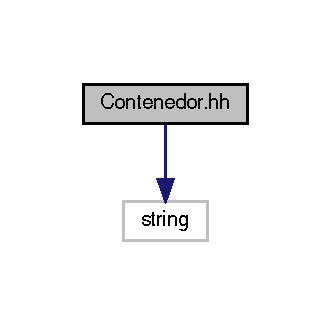
\includegraphics[width=159pt]{_contenedor_8hh__incl}
\end{center}
\end{figure}
\subsection*{Clases}
\begin{DoxyCompactItemize}
\item 
class \hyperlink{class_contenedor}{Contenedor}
\begin{DoxyCompactList}\small\item\em Representa un contenidor amb una matrícula i una longitud. \end{DoxyCompactList}\end{DoxyCompactItemize}


\subsection{Descripción detallada}
Especificació de la classe \hyperlink{class_contenedor}{Contenedor}. 


\hypertarget{pro2_8cc}{}\section{Referencia del Archivo pro2.\+cc}
\label{pro2_8cc}\index{pro2.\+cc@{pro2.\+cc}}
Dependencia gráfica adjunta para pro2.\+cc\+:
\nopagebreak
\begin{figure}[H]
\begin{center}
\leavevmode
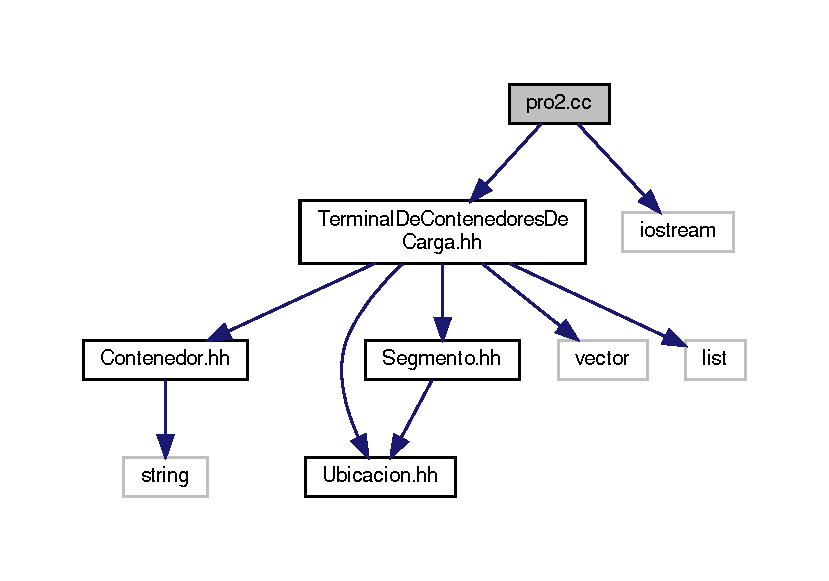
\includegraphics[width=350pt]{pro2_8cc__incl}
\end{center}
\end{figure}
\subsection*{Funciones}
\begin{DoxyCompactItemize}
\item 
int \hyperlink{pro2_8cc_ae66f6b31b5ad750f1fe042a706a4e3d4}{main} ()
\begin{DoxyCompactList}\small\item\em Programa principal para el ejercicio {\itshape Gestión de una terminal de contenedores de carga}. \end{DoxyCompactList}\end{DoxyCompactItemize}


\subsection{Documentación de las funciones}
\mbox{\Hypertarget{pro2_8cc_ae66f6b31b5ad750f1fe042a706a4e3d4}\label{pro2_8cc_ae66f6b31b5ad750f1fe042a706a4e3d4}} 
\index{pro2.\+cc@{pro2.\+cc}!main@{main}}
\index{main@{main}!pro2.\+cc@{pro2.\+cc}}
\subsubsection{\texorpdfstring{main()}{main()}}
{\footnotesize\ttfamily int main (\begin{DoxyParamCaption}{ }\end{DoxyParamCaption})}



Programa principal para el ejercicio {\itshape Gestión de una terminal de contenedores de carga}. 



Definición en la línea 21 del archivo pro2.\+cc.


\begin{DoxyCode}
21             \{
22     
23     \textcolor{keywordtype}{string} comando;
24     cin >> comando;
25     
26     \textcolor{keywordflow}{while} (comando != \textcolor{stringliteral}{"fin"}) \{
27         
28         \textcolor{keywordtype}{int} HILERAS, PLAZAS, PISOS;
29         cin >> HILERAS >> PLAZAS >> PISOS;
30         \hyperlink{class_terminal}{Terminal} terminal (HILERAS, PLAZAS, PISOS);
31         
32         cin >> comando;
33         
34         \textcolor{keywordflow}{while} (comando != \textcolor{stringliteral}{"fin"} and comando != \textcolor{stringliteral}{"crea\_terminal"}) \{
35             
36             \textcolor{keywordflow}{if} (comando == \textcolor{stringliteral}{"inserta\_contenedor"} or comando == \textcolor{stringliteral}{"i"}) \{
37                 
38                 \textcolor{keywordtype}{string} matricula;
39                 \textcolor{keywordtype}{int} longitud;
40                 cin >> matricula >> longitud;
41                 \hyperlink{class_contenedor}{Contenedor} contenedor (matricula, longitud);
42                 
43                 \textcolor{keywordflow}{if} (terminal.existe\_contenedor (matricula)) cout << \textcolor{stringliteral}{"Ya existe un contenedor con la misma
       matricula"} << endl;
44                 
45                 \textcolor{keywordflow}{else} terminal.insertar\_contenedor (contenedor);
46             \}
47             
48             \textcolor{keywordflow}{else} \textcolor{keywordflow}{if} (comando == \textcolor{stringliteral}{"retira\_contenedor"} or comando == \textcolor{stringliteral}{"r"}) \{
49                 
50                 \textcolor{keywordtype}{string} matricula;
51                 cin >> matricula;
52                 
53                 \textcolor{keywordflow}{if} (not terminal.existe\_contenedor (matricula)) cout << \textcolor{stringliteral}{"No existe un contenedor con esa
       matricula"} << endl;
54                 
55                 \textcolor{keywordflow}{else} terminal.retirar\_contenedor (matricula);
56             \}
57             
58             \textcolor{keywordflow}{else} \textcolor{keywordflow}{if} (comando == \textcolor{stringliteral}{"donde"}) \{
59                
60                 \textcolor{keywordtype}{string} matricula;
61                 cin >> matricula;
62                 
63                 \hyperlink{class_ubicacion}{Ubicacion} u;
64                 u = terminal.donde (matricula);
65                 u.\hyperlink{class_ubicacion_a6b693a32d8bbd9afce30b11d19b68846}{print}();
66             \}
67             
68             \textcolor{keywordflow}{else} \textcolor{keywordflow}{if} (comando == \textcolor{stringliteral}{"longitud"}) \{
69                 
70                 \textcolor{keywordtype}{string} matricula;
71                 cin >> matricula;
72                 
73                 \textcolor{keywordflow}{if} (not terminal.existe\_contenedor (matricula)) cout << \textcolor{stringliteral}{"No existe un contenedor con esa
       matricula"} << endl;
74                 
75                 \textcolor{keywordflow}{else} \{
76                     
77                     \textcolor{keywordtype}{int} l;
78                     l = terminal.longitud (matricula);
79                     cout << l << endl;
80                 \}
81             \}
82             
83             \textcolor{keywordflow}{else} \textcolor{keywordflow}{if} (comando == \textcolor{stringliteral}{"contenedor\_ocupa"}) \{
84                 
85                 \textcolor{keywordtype}{int} i, j, k;
86                 cin >> i >> j >> k;
87                 
88                 \textcolor{keywordflow}{if} (i < 0 or i >= HILERAS or j < 0 or j >= PLAZAS or k < 0 or k >= PISOS) cout << \textcolor{stringliteral}{"
      Ubicacion fuera del area de almacenaje"} << endl;
89                 
90                 \textcolor{keywordflow}{else} \{
91                     
92                     \hyperlink{class_ubicacion}{Ubicacion} u (i, j, k);
93                     \textcolor{keywordtype}{string} matricula;
94                     matricula = terminal.matricula (u);
95                     
96                     \textcolor{keywordflow}{if} (matricula != \textcolor{stringliteral}{"-1"}) cout << matricula << endl;
97                 \}
98             \}
99             
100             \textcolor{keywordflow}{else} \textcolor{keywordflow}{if} (comando == \textcolor{stringliteral}{"num\_hileras"}) \{
101                 
102                 \textcolor{keywordtype}{int} hileras;
103                 hileras = terminal.hileras();
104                 cout << hileras << endl;
105             \}
106             
107             \textcolor{keywordflow}{else} \textcolor{keywordflow}{if} (comando == \textcolor{stringliteral}{"num\_plazas"}) \{
108                 
109                 \textcolor{keywordtype}{int} plazas;
110                 plazas = terminal.plazas();
111                 cout << plazas << endl;
112             \}
113             
114             \textcolor{keywordflow}{else} \textcolor{keywordflow}{if} (comando == \textcolor{stringliteral}{"num\_pisos"}) \{
115                 
116                 \textcolor{keywordtype}{int} pisos;
117                 pisos = terminal.pisos();
118                 cout << pisos << endl;
119             \}
120             
121             \textcolor{keywordflow}{else} \textcolor{keywordflow}{if} (comando == \textcolor{stringliteral}{"area\_espera"}) terminal.escribir\_AreaDeEspera();
122             
123             \textcolor{keywordflow}{else} \textcolor{keywordflow}{if} (comando == \textcolor{stringliteral}{"contenedores"}) terminal.escribir\_ContenedoresAlmacenaje();
124             
125             \textcolor{keywordflow}{else} \textcolor{keywordflow}{if} (comando == \textcolor{stringliteral}{"area\_almacenaje"}) terminal.representar\_AreaDeAlmacenaje();
126             
127             \textcolor{keywordflow}{else} \textcolor{keywordflow}{if} (comando == \textcolor{stringliteral}{"huecos"}) terminal.escribir\_Huecos();
128         \}
129     \}
130 \}
\end{DoxyCode}

\hypertarget{_segmento_8hh}{}\section{Referencia del Archivo Segmento.\+hh}
\label{_segmento_8hh}\index{Segmento.\+hh@{Segmento.\+hh}}


Especificació de la classe \hyperlink{class_segmento}{Segmento}.  


Dependencia gráfica adjunta para Segmento.\+hh\+:
\nopagebreak
\begin{figure}[H]
\begin{center}
\leavevmode
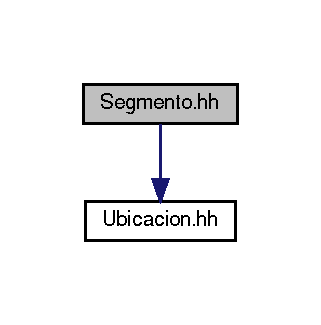
\includegraphics[width=154pt]{_segmento_8hh__incl}
\end{center}
\end{figure}
\subsection*{Clases}
\begin{DoxyCompactItemize}
\item 
class \hyperlink{class_segmento}{Segmento}
\begin{DoxyCompactList}\small\item\em Representa un segment amb una ubicació i una longitud. \end{DoxyCompactList}\end{DoxyCompactItemize}


\subsection{Descripción detallada}
Especificació de la classe \hyperlink{class_segmento}{Segmento}. 


\hypertarget{_terminal_de_contenedores_de_carga_8hh}{}\section{Referencia del Archivo Terminal\+De\+Contenedores\+De\+Carga.\+hh}
\label{_terminal_de_contenedores_de_carga_8hh}\index{Terminal\+De\+Contenedores\+De\+Carga.\+hh@{Terminal\+De\+Contenedores\+De\+Carga.\+hh}}


Especificación de la clase \hyperlink{class_terminal}{Terminal}.  


Dependencia gráfica adjunta para Terminal\+De\+Contenedores\+De\+Carga.\+hh\+:
\nopagebreak
\begin{figure}[H]
\begin{center}
\leavevmode
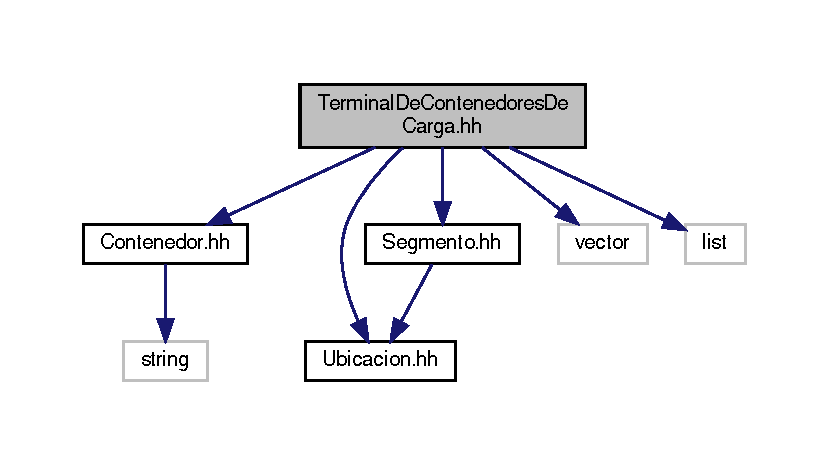
\includegraphics[width=350pt]{_terminal_de_contenedores_de_carga_8hh__incl}
\end{center}
\end{figure}
\subsection*{Clases}
\begin{DoxyCompactItemize}
\item 
class \hyperlink{class_terminal}{Terminal}
\begin{DoxyCompactList}\small\item\em Representa una \hyperlink{class_terminal}{Terminal} de contenedores de carga. \end{DoxyCompactList}\end{DoxyCompactItemize}


\subsection{Descripción detallada}
Especificación de la clase \hyperlink{class_terminal}{Terminal}. 

\begin{DoxyDate}{Fecha}
31/10/2020 
\end{DoxyDate}
\begin{DoxyAuthor}{Autor}
Pérez Castillo, Pol 
\end{DoxyAuthor}

\hypertarget{_ubicacion_8hh}{}\section{Referencia del Archivo Ubicacion.\+hh}
\label{_ubicacion_8hh}\index{Ubicacion.\+hh@{Ubicacion.\+hh}}


Especificació de la classe \hyperlink{class_ubicacion}{Ubicacion}.  


\subsection*{Clases}
\begin{DoxyCompactItemize}
\item 
class \hyperlink{class_ubicacion}{Ubicacion}
\begin{DoxyCompactList}\small\item\em Representa una ubicació en una terminal amb 3 coordenades. \end{DoxyCompactList}\end{DoxyCompactItemize}


\subsection{Descripción detallada}
Especificació de la classe \hyperlink{class_ubicacion}{Ubicacion}. 


%--- End generated contents ---

% Index
\backmatter
\newpage
\phantomsection
\clearemptydoublepage
\addcontentsline{toc}{chapter}{Índice}
\printindex

\end{document}
